% -------------------------------------------------------------------------
% ------ nuweb macros (redefine as desired, or omit with "nuweb -p") ------
% -------------------------------------------------------------------------
\providecommand{\NWtxtMacroDefBy}{Macro defined by}
\providecommand{\NWtxtMacroRefIn}{Macro referenced in}
\providecommand{\NWtxtMacroNoRef}{Macro never referenced}
\providecommand{\NWtxtDefBy}{Defined by}
\providecommand{\NWtxtRefIn}{Referenced in}
\providecommand{\NWtxtNoRef}{Not referenced}
\providecommand{\NWtxtFileDefBy}{File defined by}
\providecommand{\NWsep}{${\diamond}$}
\providecommand{\NWlink}[2]{\hyperlink{#1}{#2}}
\providecommand{\NWtarget}[2]{% move baseline up by \baselineskip 
  \raisebox{\baselineskip}[1.5ex][0ex]{%
    \mbox{%
      \hypertarget{#1}{%
        \raisebox{-1\baselineskip}[0ex][0ex]{%
          \mbox{#2}%
}}}}}
% -------------------------------------------------------------------------

\documentclass[11pt,oneside]{article}	%use"amsart"insteadof"article"forAMSLaTeXformat
\usepackage{geometry}		%Seegeometry.pdftolearnthelayoutoptions.Therearelots.
\geometry{letterpaper}		%...ora4paperora5paperor...
%\geometry{landscape}		%Activateforforrotatedpagegeometry
%\usepackage[parfill]{parskip}		%Activatetobeginparagraphswithanemptylineratherthananindent
\usepackage{graphicx}				%Usepdf,png,jpg,orepsßwithpdflatex;useepsinDVImode
								%TeXwillautomaticallyconverteps-->pdfinpdflatex		
\usepackage{amssymb}
\usepackage{amsmath}
\usepackage{amsthm}
\newtheorem{definition}{Definition}
\newtheorem{theorem}{Theorem}
\newtheorem{example}{Example}
\usepackage[colorlinks]{hyperref}

%----macros begin---------------------------------------------------------------
\usepackage{color}
\usepackage{amsthm}

\def\conv{\mbox{\textrm{conv}\,}}
\def\aff{\mbox{\textrm{aff}\,}}
\def\E{\mathbb{E}}
\def\R{\mathbb{R}}
\def\Z{\mathbb{Z}}
\def\tex{\TeX}
\def\latex{\LaTeX}
\def\v#1{{\bf #1}}
\def\p#1{{\bf #1}}
\def\T#1{{\bf #1}}

\def\vet#1{{\left(\begin{array}{cccccccccccccccccccc}#1\end{array}\right)}}
\def\mat#1{{\left(\begin{array}{cccccccccccccccccccc}#1\end{array}\right)}}

\def\lin{\mbox{\rm lin}\,}
\def\aff{\mbox{\rm aff}\,}
\def\pos{\mbox{\rm pos}\,}
\def\cone{\mbox{\rm cone}\,}
\def\conv{\mbox{\rm conv}\,}
\newcommand{\homog}[0]{\mbox{\rm homog}\,}
\newcommand{\relint}[0]{\mbox{\rm relint}\,}

%----macros end-----------------------------------------------------------------

\title{The basic \texttt{larcc} module
\footnote{This document is part of the \emph{Linear Algebraic Representation with CoChains} (LAR-CC) framework~\cite{cclar-proj:2013:00}. \today}
}
\author{The LARCC team}
%\date{}							%Activatetodisplayagivendateornodate

\begin{document}
\maketitle
\nonstopmode

\tableofcontents
\newpage


\section{Basic representations}

A few basic representation of topology are used in LARCC. They include some common sparse matrix representations: CSR (Compressed Sparse Row),  CSC (Compressed Sparse Column),   COO (Coordinate Representation), and BRC (Binary Row Compressed). 

\subsection{BRC (Binary Row Compressed)}

We denote as BRC (Binary Row Compressed) the standard input representation of our LARCC framework. A BRC representation is an array of arrays of integers, with no requirement of equal length for the component arrays. The BRC format is used to represent a (normally sparse) binary matrix. Each component array corresponds to a matrix row, and contains the indices of columns that store a 1 value. No storage is used for 0 values.

\paragraph{BRC format example}

Let $A = (a_{i,j} \in \{0,1\})$ be a binary matrix. The notation $\texttt{BRC}(A)$ is used for the corresponding data structure.
\[
A = \mat{
0,1,0,0,0,0,0,1,0,0\\
0,0,1,0,0,0,0,0,0,0\\
1,0,0,1,0,0,0,0,0,1\\
1,0,0,0,0,0,1,0,0,0\\
0,0,0,0,0,1,1,1,0,0\\
0,0,1,0,1,0,0,0,1,0\\
0,0,0,0,0,0,0,0,0,0\\
0,1,0,0,0,0,0,1,0,1\\
0,0,0,1,0,0,0,0,1,0\\
0,1,1,0,1,0,0,0,0,0\\
}
\qquad\mapsto\qquad \texttt{BRC}(A) =
\begin{minipage}[c]{5cm}
\begin{verbatim}
[[1,7],
 [2],
 [0,3,9],
 [0,6],
 [5,6,7],
 [2,4,8],
 [],
 [1,7,9],
 [3,8],
 [1,2,4]]
\end{verbatim}
\end{minipage}
\]


\subsection{Format conversions}

First we give the function \texttt{triples2mat} to make the transformation from the sparse matrix, given as a list of triples \emph{row,column,value} (non-zero elements), to the \texttt{scipy.sparse} format corresponding to the \texttt{shape} parameter, set by default to \texttt{"csr"}, that stands for \emph{Compressed Sparse Row}, the normal matrix format of the LARCC framework. 
%-------------------------------------------------------------------------------
\begin{flushleft} \small
\begin{minipage}{\linewidth} \label{scrap1}
\protect\makebox[0ex][r]{\NWtarget{nuweb3a}{\rule{0ex}{0ex}}\hspace{1em}}$\langle\,$From list of triples to scipy.sparse\nobreak\ {\footnotesize 3a}$\,\rangle\equiv$
\vspace{-1ex}
\begin{list}{}{} \item
\mbox{}\verb@def triples2mat(triples,shape="csr"):@\\
\mbox{}\verb@    n = len(triples)@\\
\mbox{}\verb@    data = arange(n)@\\
\mbox{}\verb@    ij = arange(2*n).reshape(2,n)@\\
\mbox{}\verb@    for k,item in enumerate(triples):@\\
\mbox{}\verb@        ij[0][k],ij[1][k],data[k] = item@\\
\mbox{}\verb@    return scipy.sparse.coo_matrix((data, ij)).asformat(shape)@\\
\mbox{}\verb@@{\NWsep}
\end{list}
\vspace{-1ex}
\footnotesize\addtolength{\baselineskip}{-1ex}
\begin{list}{}{\setlength{\itemsep}{-\parsep}\setlength{\itemindent}{-\leftmargin}}
\item \NWtxtMacroRefIn\ \NWlink{nuweb19a}{19a}.
\end{list}
\end{minipage}\\[4ex]
\end{flushleft}
%-------------------------------------------------------------------------------
The function \texttt{brc2Coo} transforms a \texttt{BRC} representation in a list of triples (\emph{row}, \emph{column}, 1) ordered by row.
%-------------------------------------------------------------------------------
\begin{flushleft} \small
\begin{minipage}{\linewidth} \label{scrap2}
\protect\makebox[0ex][r]{\NWtarget{nuweb3b}{\rule{0ex}{0ex}}\hspace{1em}}$\langle\,$Brc to Coo transformation\nobreak\ {\footnotesize 3b}$\,\rangle\equiv$
\vspace{-1ex}
\begin{list}{}{} \item
\mbox{}\verb@def brc2Coo(ListOfListOfInt):@\\
\mbox{}\verb@    COOm = [[k,col,1] for k,row in enumerate(ListOfListOfInt)@\\
\mbox{}\verb@            for col in row ]@\\
\mbox{}\verb@    return COOm@\\
\mbox{}\verb@@{\NWsep}
\end{list}
\vspace{-1ex}
\footnotesize\addtolength{\baselineskip}{-1ex}
\begin{list}{}{\setlength{\itemsep}{-\parsep}\setlength{\itemindent}{-\leftmargin}}
\item \NWtxtMacroRefIn\ \NWlink{nuweb19a}{19a}.
\end{list}
\end{minipage}\\[4ex]
\end{flushleft}
%-------------------------------------------------------------------------------

Two coordinate compressed sparse matrices \texttt{cooFV} and \texttt{cooEV} are created below, starting from the \texttt{BRC} representation \texttt{FV} and \texttt{EV} of the incidence of vertices on faces and edges, respectively, for a very simple plane triangulation.
%-------------------------------------------------------------------------------
\begin{flushleft} \small
\begin{minipage}{\linewidth} \label{scrap3}
\protect\makebox[0ex][r]{\NWtarget{nuweb3c}{\rule{0ex}{0ex}}\hspace{1em}}$\langle\,$Test example of Brc to Coo transformation\nobreak\ {\footnotesize 3c}$\,\rangle\equiv$
\vspace{-1ex}
\begin{list}{}{} \item
\mbox{}\verb@print "\n>>> brc2Coo"@\\
\mbox{}\verb@V = [[0, 0], [1, 0], [2, 0], [0, 1], [1, 1], [2, 1]]@\\
\mbox{}\verb@FV = [[0, 1, 3], [1, 2, 4], [1, 3, 4], [2, 4, 5]]@\\
\mbox{}\verb@EV = [[0,1],[0,3],[1,2],[1,3],[1,4],[2,4],[2,5],[3,4],[4,5]]@\\
\mbox{}\verb@cooFV = brc2Coo(FV)@\\
\mbox{}\verb@cooEV = brc2Coo(EV)@\\
\mbox{}\verb@assert cooFV == [[0,0,1],[0,1,1],[0,3,1],[1,1,1],[1,2,1],[1,4,1],[2,1,1],@\\
\mbox{}\verb@[2,3,1], [2,4,1],[3,2,1],[3,4,1],[3,5,1]]@\\
\mbox{}\verb@assert cooEV == [[0,0,1],[0,1,1],[1,0,1],[1,3,1],[2,1,1],[2,2,1],[3,1,1],@\\
\mbox{}\verb@[3,3,1],[4,1,1],[4,4,1],[5,2,1],[5,4,1],[6,2,1],[6,5,1],[7,3,1],[7,4,1],@\\
\mbox{}\verb@[8,4,1],[8,5,1]]@\\
\mbox{}\verb@@{\NWsep}
\end{list}
\vspace{-1ex}
\footnotesize\addtolength{\baselineskip}{-1ex}
\begin{list}{}{\setlength{\itemsep}{-\parsep}\setlength{\itemindent}{-\leftmargin}}
\item \NWtxtMacroRefIn\ \NWlink{nuweb19b}{19b}.
\end{list}
\end{minipage}\\[4ex]
\end{flushleft}
%-------------------------------------------------------------------------------
%-------------------------------------------------------------------------------
\begin{flushleft} \small
\begin{minipage}{\linewidth} \label{scrap4}
\protect\makebox[0ex][r]{\NWtarget{nuweb4a}{\rule{0ex}{0ex}}\hspace{1em}}$\langle\,$Coo to Csr transformation\nobreak\ {\footnotesize 4a}$\,\rangle\equiv$
\vspace{-1ex}
\begin{list}{}{} \item
\mbox{}\verb@def coo2Csr(COOm):@\\
\mbox{}\verb@    CSRm = triples2mat(COOm,"csr")@\\
\mbox{}\verb@    return CSRm@\\
\mbox{}\verb@@{\NWsep}
\end{list}
\vspace{-1ex}
\footnotesize\addtolength{\baselineskip}{-1ex}
\begin{list}{}{\setlength{\itemsep}{-\parsep}\setlength{\itemindent}{-\leftmargin}}
\item \NWtxtMacroRefIn\ \NWlink{nuweb19a}{19a}.
\end{list}
\end{minipage}\\[4ex]
\end{flushleft}
%-------------------------------------------------------------------------------

Two CSR sparse matrices \texttt{csrFV} and \texttt{csrEV} are generated (by \emph{scipy.sparse})  in the following example:
%-------------------------------------------------------------------------------
\begin{flushleft} \small
\begin{minipage}{\linewidth} \label{scrap5}
\protect\makebox[0ex][r]{\NWtarget{nuweb4b}{\rule{0ex}{0ex}}\hspace{1em}}$\langle\,$Test example of Coo to Csr transformation\nobreak\ {\footnotesize 4b}$\,\rangle\equiv$
\vspace{-1ex}
\begin{list}{}{} \item
\mbox{}\verb@csrFV = coo2Csr(cooFV)@\\
\mbox{}\verb@csrEV = coo2Csr(cooEV)@\\
\mbox{}\verb@print "\ncsr(FV) =\n", repr(csrFV)@\\
\mbox{}\verb@print "\ncsr(EV) =\n", repr(csrEV)@\\
\mbox{}\verb@@{\NWsep}
\end{list}
\vspace{-1ex}
\footnotesize\addtolength{\baselineskip}{-1ex}
\begin{list}{}{\setlength{\itemsep}{-\parsep}\setlength{\itemindent}{-\leftmargin}}
\item \NWtxtMacroRefIn\ \NWlink{nuweb19b}{19b}.
\end{list}
\end{minipage}\\[4ex]
\end{flushleft}
%-------------------------------------------------------------------------------
The \emph{scipy} printout of the last two lines above is the following:
%-------------------------------------------------------------------------------
{\small
\begin{verbatim}
csr(FV) = <4x6 sparse matrix of type '<type 'numpy.int64'>'
		   with 12 stored elements in Compressed Sparse Row format>
csr(EV) = <9x6 sparse matrix of type '<type 'numpy.int64'>'
		   with 18 stored elements in Compressed Sparse Row format>
\end{verbatim}}
%-------------------------------------------------------------------------------
The transformation from BRC to CSR format is implemented slightly differently, according to the fact that the matrix dimension is either unknown (\texttt{shape=(0,0)}) or known.
%-------------------------------------------------------------------------------
\begin{flushleft} \small
\begin{minipage}{\linewidth} \label{scrap6}
\protect\makebox[0ex][r]{\NWtarget{nuweb4c}{\rule{0ex}{0ex}}\hspace{1em}}$\langle\,$Brc to Csr transformation\nobreak\ {\footnotesize 4c}$\,\rangle\equiv$
\vspace{-1ex}
\begin{list}{}{} \item
\mbox{}\verb@def csrCreate(BRCmatrix,shape=(0,0)):@\\
\mbox{}\verb@    triples = brc2Coo(BRCmatrix)@\\
\mbox{}\verb@    if shape == (0,0):@\\
\mbox{}\verb@        CSRmatrix = coo2Csr(triples)@\\
\mbox{}\verb@    else:@\\
\mbox{}\verb@        CSRmatrix = scipy.sparse.csr_matrix(shape)@\\
\mbox{}\verb@        for i,j,v in triples: CSRmatrix[i,j] = v@\\
\mbox{}\verb@    return CSRmatrix@\\
\mbox{}\verb@@{\NWsep}
\end{list}
\vspace{-1ex}
\footnotesize\addtolength{\baselineskip}{-1ex}
\begin{list}{}{\setlength{\itemsep}{-\parsep}\setlength{\itemindent}{-\leftmargin}}
\item \NWtxtMacroRefIn\ \NWlink{nuweb19a}{19a}.
\end{list}
\end{minipage}\\[4ex]
\end{flushleft}
%-------------------------------------------------------------------------------
The conversion to CSR format of the characteristic matrix \emph{faces-vertices} \texttt{FV} is given below for our simple example made by four triangle of a manifold 2D space, graphically shown in Figure~\ref{fig:2D-non-manifold}a. The LAR representation with CSR matrices does not make difference between manifolds and non-manifolds, conversely than most modern solid modelling representation schemes, as shown by removing from \texttt{FV} the third triangle, giving the model in Figure~\ref{fig:2D-non-manifold}b.
%-------------------------------------------------------------------------------
\begin{flushleft} \small
\begin{minipage}{\linewidth} \label{scrap7}
\protect\makebox[0ex][r]{\NWtarget{nuweb5a}{\rule{0ex}{0ex}}\hspace{1em}}$\langle\,$Test example of Brc to Csr transformation\nobreak\ {\footnotesize 5a}$\,\rangle\equiv$
\vspace{-1ex}
\begin{list}{}{} \item
\mbox{}\verb@print "\n>>> brc2Csr"@\\
\mbox{}\verb@V = [[0, 0], [1, 0], [2, 0], [0, 1], [1, 1], [2, 1]]@\\
\mbox{}\verb@FV = [[0, 1, 3], [1, 2, 4], [1, 3, 4], [2, 4, 5]]@\\
\mbox{}\verb@EV = [[0,1],[0,3],[1,2],[1,3],[1,4],[2,4],[2,5],[3,4],[4,5]]@\\
\mbox{}\verb@csrFV = csrCreate(FV)@\\
\mbox{}\verb@csrEV = csrCreate(EV)@\\
\mbox{}\verb@print "\ncsrCreate(FV) =\n", csrFV@\\
\mbox{}\verb@VIEW(STRUCT(MKPOLS((V,FV))))@\\
\mbox{}\verb@VIEW(STRUCT(MKPOLS((V,EV))))@\\
\mbox{}\verb@@{\NWsep}
\end{list}
\vspace{-1ex}
\footnotesize\addtolength{\baselineskip}{-1ex}
\begin{list}{}{\setlength{\itemsep}{-\parsep}\setlength{\itemindent}{-\leftmargin}}
\item \NWtxtMacroRefIn\ \NWlink{nuweb6d}{6d}\NWlink{nuweb19b}{, 19b}.
\end{list}
\end{minipage}\\[4ex]
\end{flushleft}
%-------------------------------------------------------------------------------

\begin{figure}[htbp] %  figure placement: here, top, bottom, or page
   \centering
   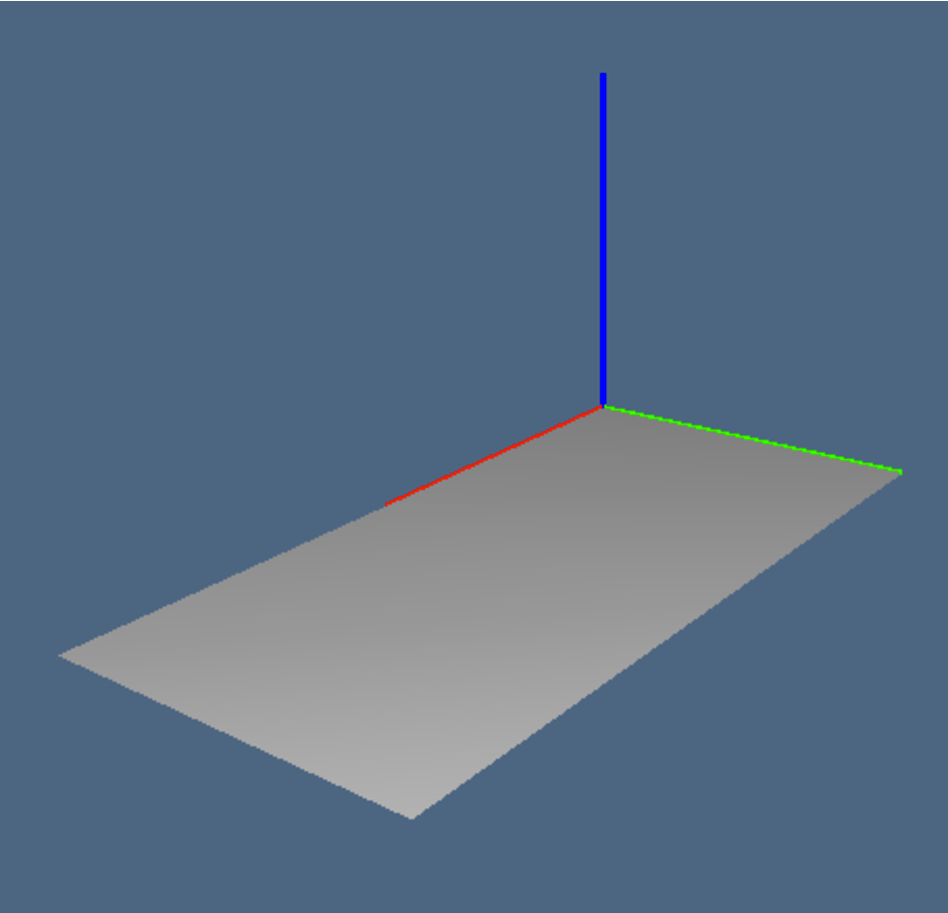
\includegraphics[height=0.25\linewidth,width=0.25\linewidth]{images/2D-non-manifold-a} 
   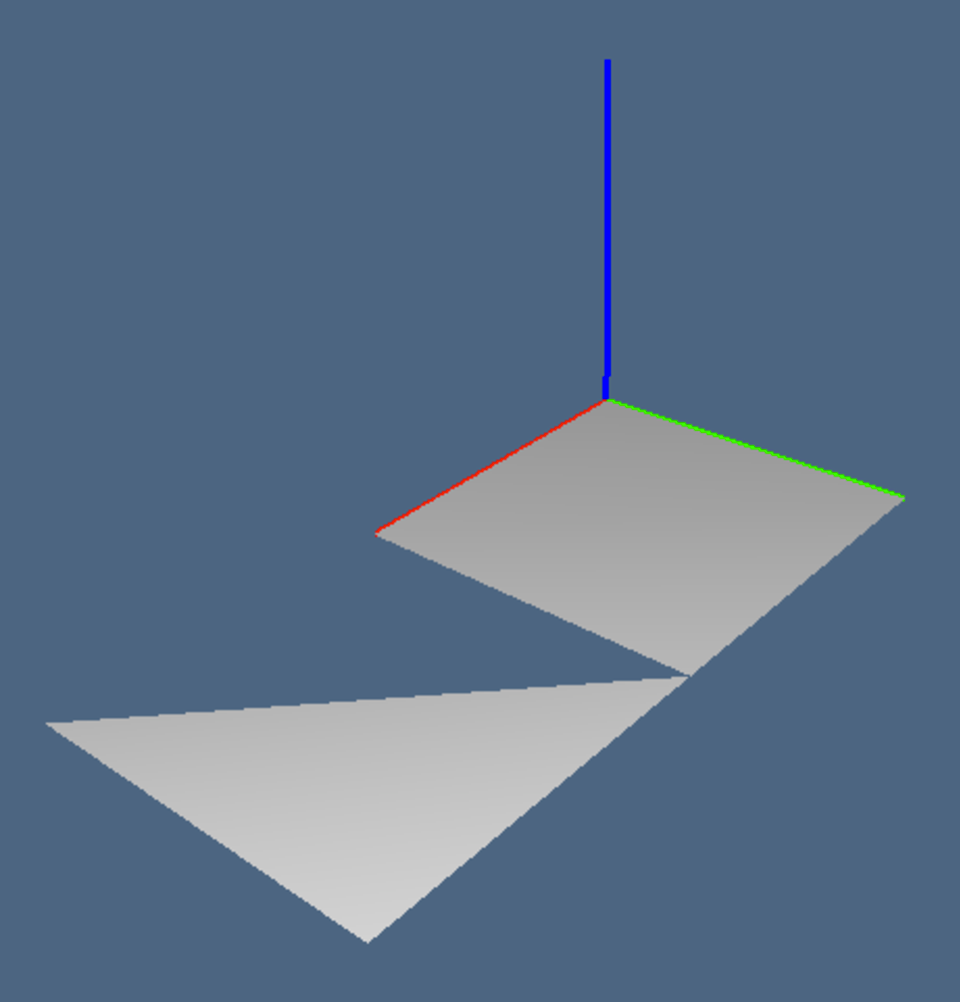
\includegraphics[height=0.25\linewidth,width=0.25\linewidth]{images/2D-non-manifold-b} 
   \caption{(a) Manifold two-dimensional space; (b) non-manifold space.}
   \label{fig:2D-non-manifold}
\end{figure}

\section{Matrix operations}

As we know, the LAR representation of topology is based on CSR representation of sparse binary (and integer) matrices.
Two Utility functions allow to query the number of rows and columns of a CSR matrix, independently from the low-level implementation (that in the following is provided by \emph{scipy.sparse}).
%-------------------------------------------------------------------------------
\begin{flushleft} \small
\begin{minipage}{\linewidth} \label{scrap8}
\protect\makebox[0ex][r]{\NWtarget{nuweb5b}{\rule{0ex}{0ex}}\hspace{1em}}$\langle\,$Query Matrix shape\nobreak\ {\footnotesize 5b}$\,\rangle\equiv$
\vspace{-1ex}
\begin{list}{}{} \item
\mbox{}\verb@def csrGetNumberOfRows(CSRmatrix):@\\
\mbox{}\verb@    Int = CSRmatrix.shape[0]@\\
\mbox{}\verb@    return Int@\\
\mbox{}\verb@    @\\
\mbox{}\verb@def csrGetNumberOfColumns(CSRmatrix):@\\
\mbox{}\verb@    Int = CSRmatrix.shape[1]@\\
\mbox{}\verb@    return Int@\\
\mbox{}\verb@@{\NWsep}
\end{list}
\vspace{-1ex}
\footnotesize\addtolength{\baselineskip}{-1ex}
\begin{list}{}{\setlength{\itemsep}{-\parsep}\setlength{\itemindent}{-\leftmargin}}
\item \NWtxtMacroRefIn\ \NWlink{nuweb19a}{19a}.
\end{list}
\end{minipage}\\[4ex]
\end{flushleft}
%-------------------------------------------------------------------------------
%-------------------------------------------------------------------------------
\begin{flushleft} \small
\begin{minipage}{\linewidth} \label{scrap9}
\protect\makebox[0ex][r]{\NWtarget{nuweb6a}{\rule{0ex}{0ex}}\hspace{1em}}$\langle\,$Test examples of Query Matrix shape\nobreak\ {\footnotesize 6a}$\,\rangle\equiv$
\vspace{-1ex}
\begin{list}{}{} \item
\mbox{}\verb@print "\n>>> csrGetNumberOfRows"@\\
\mbox{}\verb@print "\ncsrGetNumberOfRows(csrFV) =", csrGetNumberOfRows(csrFV)@\\
\mbox{}\verb@print "\ncsrGetNumberOfRows(csrEV) =", csrGetNumberOfRows(csrEV)@\\
\mbox{}\verb@print "\n>>> csrGetNumberOfColumns"@\\
\mbox{}\verb@print "\ncsrGetNumberOfColumns(csrFV) =", csrGetNumberOfColumns(csrFV)@\\
\mbox{}\verb@print "\ncsrGetNumberOfColumns(csrEV) =", csrGetNumberOfColumns(csrEV)@\\
\mbox{}\verb@@{\NWsep}
\end{list}
\vspace{-1ex}
\footnotesize\addtolength{\baselineskip}{-1ex}
\begin{list}{}{\setlength{\itemsep}{-\parsep}\setlength{\itemindent}{-\leftmargin}}
\item \NWtxtMacroRefIn\ \NWlink{nuweb19b}{19b}.
\end{list}
\end{minipage}\\[4ex]
\end{flushleft}
%-------------------------------------------------------------------------------

\paragraph{}

%-------------------------------------------------------------------------------
\begin{flushleft} \small
\begin{minipage}{\linewidth} \label{scrap10}
\protect\makebox[0ex][r]{\NWtarget{nuweb6b}{\rule{0ex}{0ex}}\hspace{1em}}$\langle\,$Sparse to dense matrix transformation\nobreak\ {\footnotesize 6b}$\,\rangle\equiv$
\vspace{-1ex}
\begin{list}{}{} \item
\mbox{}\verb@def csr2DenseMatrix(CSRm):@\\
\mbox{}\verb@    nrows = csrGetNumberOfRows(CSRm)@\\
\mbox{}\verb@    ncolumns = csrGetNumberOfColumns(CSRm)@\\
\mbox{}\verb@    ScipyMat = zeros((nrows,ncolumns),int)@\\
\mbox{}\verb@    C = CSRm.tocoo()@\\
\mbox{}\verb@    for triple in zip(C.row,C.col,C.data):@\\
\mbox{}\verb@        ScipyMat[triple[0],triple[1]] = triple[2]@\\
\mbox{}\verb@    return ScipyMat@\\
\mbox{}\verb@@{\NWsep}
\end{list}
\vspace{-1ex}
\footnotesize\addtolength{\baselineskip}{-1ex}
\begin{list}{}{\setlength{\itemsep}{-\parsep}\setlength{\itemindent}{-\leftmargin}}
\item \NWtxtMacroRefIn\ \NWlink{nuweb19a}{19a}.
\end{list}
\end{minipage}\\[4ex]
\end{flushleft}
%-------------------------------------------------------------------------------
%-------------------------------------------------------------------------------
\begin{flushleft} \small
\begin{minipage}{\linewidth} \label{scrap11}
\protect\makebox[0ex][r]{\NWtarget{nuweb6c}{\rule{0ex}{0ex}}\hspace{1em}}$\langle\,$Test examples of Sparse to dense matrix transformation\nobreak\ {\footnotesize 6c}$\,\rangle\equiv$
\vspace{-1ex}
\begin{list}{}{} \item
\mbox{}\verb@print "\n>>> csr2DenseMatrix"@\\
\mbox{}\verb@print "\nFV =\n", csr2DenseMatrix(csrFV)@\\
\mbox{}\verb@print "\nEV =\n", csr2DenseMatrix(csrEV)@\\
\mbox{}\verb@@{\NWsep}
\end{list}
\vspace{-1ex}
\footnotesize\addtolength{\baselineskip}{-1ex}
\begin{list}{}{\setlength{\itemsep}{-\parsep}\setlength{\itemindent}{-\leftmargin}}
\item \NWtxtMacroRefIn\ \NWlink{nuweb6d}{6d}\NWlink{nuweb19b}{, 19b}.
\end{list}
\end{minipage}\\[4ex]
\end{flushleft}
%-------------------------------------------------------------------------------

\paragraph{Characteristic matrices}
Let us compute and show in dense form the characteristic matrices of 2- and 1-cells of the simple manifold just defined.
By running the file \texttt{test/py/larcc/ex8.py} the reader will get the two matrices shown in Example~\ref{ex:denseMat}
%-------------------------------------------------------------------------------
\begin{flushleft} \small
\begin{minipage}{\linewidth} \label{scrap12}
\protect\makebox[0ex][r]{\NWtarget{nuweb6d}{\rule{0ex}{0ex}}\hspace{1em}}\verb@"test/py/larcc/ex8.py"@\nobreak\ {\footnotesize 6d }$\equiv$
\vspace{-1ex}
\begin{list}{}{} \item
\mbox{}\verb@from larcc import *@\\
\mbox{}\verb@@\hbox{$\langle\,$Test example of Brc to Csr transformation\nobreak\ {\footnotesize \NWlink{nuweb5a}{5a}}$\,\rangle$}\verb@@\\
\mbox{}\verb@@\hbox{$\langle\,$Test examples of Sparse to dense matrix transformation\nobreak\ {\footnotesize \NWlink{nuweb6c}{6c}}$\,\rangle$}\verb@@\\
\mbox{}\verb@@{\NWsep}
\end{list}
\vspace{-2ex}
\end{minipage}\\[4ex]
\end{flushleft}
%-------------------------------------------------------------------------------
 
\begin{example}[Dense Characteristic matrices]\label{ex:denseMat}
Let us notice that the two matrices below have the some numbers of columns (indexed by vertices of the cell decomposition).
This very fact allows to multiply one matrix for the other transposed, and hence to compute the matrix form of linear operators between the spaces of cells of various dimensions.
\[
\texttt{FV} =
\begin{minipage}[c]{0.29\linewidth}
\begin{verbatim}
[[1 1 0 1 0 0]
 [0 1 1 0 1 0]
 [0 1 0 1 1 0]
 [0 0 1 0 1 1]]
\end{verbatim}
\end{minipage}
\qquad
\texttt{EV} =
\begin{minipage}[c]{0.29\linewidth}
\begin{verbatim}
[[1 1 0 0 0 0]
 [1 0 0 1 0 0]
 [0 1 1 0 0 0]
 [0 1 0 1 0 0]
 [0 1 0 0 1 0]
 [0 0 1 0 1 0]
 [0 0 1 0 0 1]
 [0 0 0 1 1 0]
 [0 0 0 0 1 1]]
\end{verbatim}
\end{minipage}
\]
\end{example}

\paragraph{Matrix product and transposition}

The following macro provides the IDE interface for the two main matrix operations required by LARCC, the binary product of compatible matrices and the unary transposition of matrices.

%-------------------------------------------------------------------------------
\begin{flushleft} \small
\begin{minipage}{\linewidth} \label{scrap13}
\protect\makebox[0ex][r]{\NWtarget{nuweb7}{\rule{0ex}{0ex}}\hspace{1em}}$\langle\,$Matrix product and transposition\nobreak\ {\footnotesize 7}$\,\rangle\equiv$
\vspace{-1ex}
\begin{list}{}{} \item
\mbox{}\verb@def matrixProduct(CSRm1,CSRm2):@\\
\mbox{}\verb@    CSRm = CSRm1 * CSRm2@\\
\mbox{}\verb@    return CSRm@\\
\mbox{}\verb@@\\
\mbox{}\verb@def csrTranspose(CSRm):@\\
\mbox{}\verb@    CSRm = CSRm.T@\\
\mbox{}\verb@    return CSRm@\\
\mbox{}\verb@@{\NWsep}
\end{list}
\vspace{-1ex}
\footnotesize\addtolength{\baselineskip}{-1ex}
\begin{list}{}{\setlength{\itemsep}{-\parsep}\setlength{\itemindent}{-\leftmargin}}
\item \NWtxtMacroRefIn\ \NWlink{nuweb19a}{19a}.
\end{list}
\end{minipage}\\[4ex]
\end{flushleft}
%-------------------------------------------------------------------------------

\begin{example}[Operators from edges to faces and vice-versa]\label{ex:denseMat}
As a general rule for operators between two spaces of chains of different dimensions supported by the \emph{same} cellular complex, we use names made by two characters, whose first letter correspond to the target space, and whose second letter to the domain space. Hence \texttt{FE} must be read as the operator from edges to faces. Of course, since this use correspond to see the first letter as the space generated by rows, and the second letter as the space generated by columns. Notice that the element $(i,j)$ of such matrices stores the number of vertices shared between the (row-)cell $i$ and the (column-)cell $j$.
\[
\texttt{FE} = \texttt{FV}\ \texttt{EV}^\top = 
\begin{minipage}[c]{0.29\linewidth}
\begin{verbatim}
[[2 2 1 2 1 0 0 1 0]
 [1 0 2 1 2 2 1 1 1]
 [1 1 1 2 2 1 0 2 1]
 [0 0 1 0 1 2 2 1 2]]
\end{verbatim}
\end{minipage}
\qquad
\texttt{EF} = \texttt{EV}\ \texttt{FV}^\top = 
\begin{minipage}[c]{0.29\linewidth}
\begin{verbatim}
[[2 1 1 0]
 [2 0 1 0]
 [1 2 1 1]
 [2 1 2 0]
 [1 2 2 1]
 [0 2 1 2]
 [0 1 0 2]
 [1 1 2 1]
 [0 1 1 2]]
\end{verbatim}
\end{minipage}
\]
\end{example}

\begin{figure}[htbp] %  figure placement: here, top, bottom, or page
   \centering
   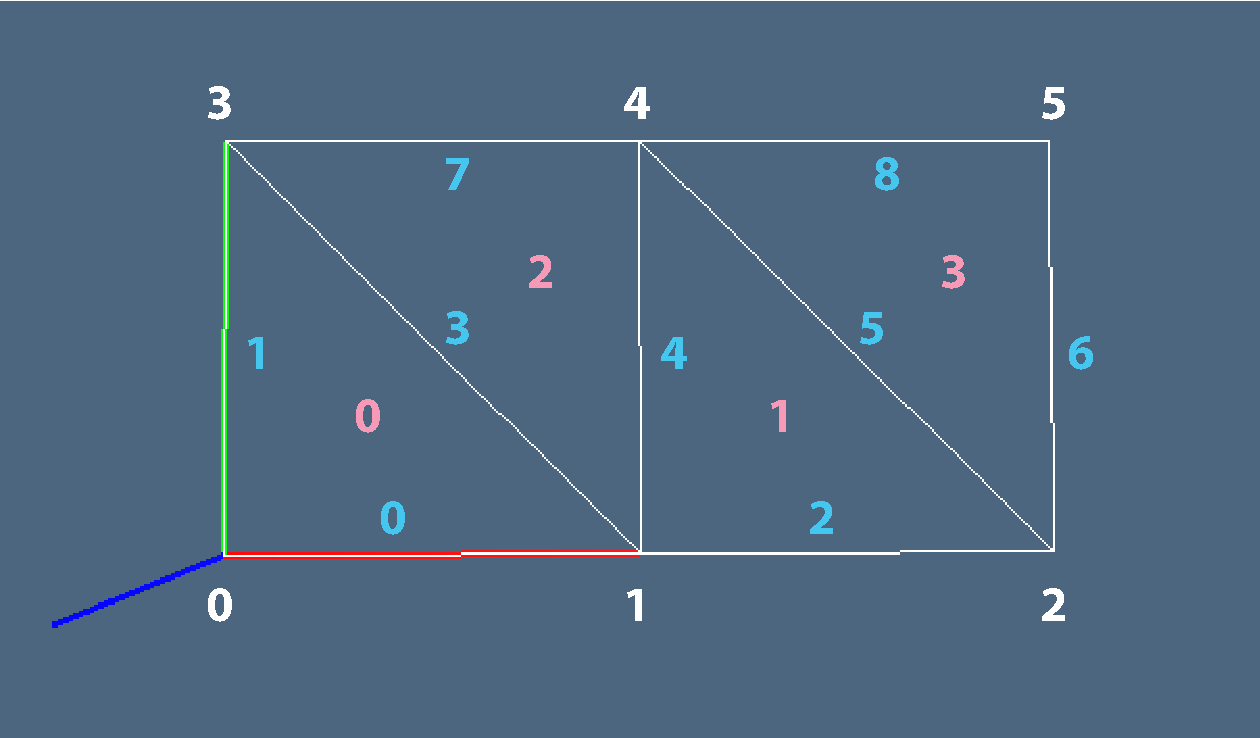
\includegraphics[width=0.6\linewidth]{images/2complex} 
   \caption{example caption}
   \label{fig:2complex}
\end{figure}
%-------------------------------------------------------------------------------
\begin{flushleft} \small
\begin{minipage}{\linewidth} \label{scrap14}
\protect\makebox[0ex][r]{\NWtarget{nuweb8}{\rule{0ex}{0ex}}\hspace{1em}}$\langle\,$Matrix filtering to produce the boundary matrix\nobreak\ {\footnotesize 8}$\,\rangle\equiv$
\vspace{-1ex}
\begin{list}{}{} \item
\mbox{}\verb@def csrBoundaryFilter(CSRm, facetLengths):@\\
\mbox{}\verb@    maxs = [max(CSRm[k].data) for k in range(CSRm.shape[0])]@\\
\mbox{}\verb@    inputShape = CSRm.shape@\\
\mbox{}\verb@    coo = CSRm.tocoo()@\\
\mbox{}\verb@    for k in range(len(coo.data)):@\\
\mbox{}\verb@        if coo.data[k]==maxs[coo.row[k]]: coo.data[k] = 1@\\
\mbox{}\verb@        else: coo.data[k] = 0@\\
\mbox{}\verb@    mtx = coo_matrix((coo.data, (coo.row, coo.col)), shape=inputShape)@\\
\mbox{}\verb@    out = mtx.tocsr()@\\
\mbox{}\verb@    return out@\\
\mbox{}\verb@@{\NWsep}
\end{list}
\vspace{-1ex}
\footnotesize\addtolength{\baselineskip}{-1ex}
\begin{list}{}{\setlength{\itemsep}{-\parsep}\setlength{\itemindent}{-\leftmargin}}
\item \NWtxtMacroRefIn\ \NWlink{nuweb19a}{19a}.
\end{list}
\end{minipage}\\[4ex]
\end{flushleft}
%-------------------------------------------------------------------------------
%-------------------------------------------------------------------------------
\begin{flushleft} \small
\begin{minipage}{\linewidth} \label{scrap15}
\protect\makebox[0ex][r]{\NWtarget{nuweb9a}{\rule{0ex}{0ex}}\hspace{1em}}$\langle\,$Test example of Matrix filtering to produce the boundary matrix\nobreak\ {\footnotesize 9a}$\,\rangle\equiv$
\vspace{-1ex}
\begin{list}{}{} \item
\mbox{}\verb@print "\n>>> csrBoundaryFilter"@\\
\mbox{}\verb@csrEF = matrixProduct(csrFV, csrTranspose(csrEV)).T@\\
\mbox{}\verb@facetLengths = [csrCell.getnnz() for csrCell in csrEV]@\\
\mbox{}\verb@CSRm = csrBoundaryFilter(csrEF, facetLengths).T@\\
\mbox{}\verb@print "\ncsrMaxFilter(csrFE) =\n", csr2DenseMatrix(CSRm)@\\
\mbox{}\verb@@{\NWsep}
\end{list}
\vspace{-1ex}
\footnotesize\addtolength{\baselineskip}{-1ex}
\begin{list}{}{\setlength{\itemsep}{-\parsep}\setlength{\itemindent}{-\leftmargin}}
\item \NWtxtMacroRefIn\ \NWlink{nuweb19b}{19b}.
\end{list}
\end{minipage}\\[4ex]
\end{flushleft}
%-------------------------------------------------------------------------------
%-------------------------------------------------------------------------------
\begin{flushleft} \small
\begin{minipage}{\linewidth} \label{scrap16}
\protect\makebox[0ex][r]{\NWtarget{nuweb9b}{\rule{0ex}{0ex}}\hspace{1em}}$\langle\,$Matrix filtering via a generic predicate\nobreak\ {\footnotesize 9b}$\,\rangle\equiv$
\vspace{-1ex}
\begin{list}{}{} \item
\mbox{}\verb@def csrPredFilter(CSRm, pred):@\\
\mbox{}\verb@   # can be done in parallel (by rows)@\\
\mbox{}\verb@   coo = CSRm.tocoo()@\\
\mbox{}\verb@   triples = [[row,col,val] for row,col,val @\\
\mbox{}\verb@            in zip(coo.row,coo.col,coo.data) if pred(val)]@\\
\mbox{}\verb@   i, j, data = TRANS(triples)@\\
\mbox{}\verb@   CSRm = scipy.sparse.coo_matrix((data,(i,j)),CSRm.shape).tocsr()@\\
\mbox{}\verb@   return CSRm@\\
\mbox{}\verb@@{\NWsep}
\end{list}
\vspace{-1ex}
\footnotesize\addtolength{\baselineskip}{-1ex}
\begin{list}{}{\setlength{\itemsep}{-\parsep}\setlength{\itemindent}{-\leftmargin}}
\item \NWtxtMacroRefIn\ \NWlink{nuweb19a}{19a}.
\end{list}
\end{minipage}\\[4ex]
\end{flushleft}
%-------------------------------------------------------------------------------
%-------------------------------------------------------------------------------
\begin{flushleft} \small
\begin{minipage}{\linewidth} \label{scrap17}
\protect\makebox[0ex][r]{\NWtarget{nuweb9c}{\rule{0ex}{0ex}}\hspace{1em}}$\langle\,$Test example of Matrix filtering via a generic predicate\nobreak\ {\footnotesize 9c}$\,\rangle\equiv$
\vspace{-1ex}
\begin{list}{}{} \item
\mbox{}\verb@print "\n>>> csrPredFilter"@\\
\mbox{}\verb@CSRm = csrPredFilter(matrixProduct(csrFV, csrTranspose(csrEV)).T, GE(2)).T@\\
\mbox{}\verb@print "\nccsrPredFilter(csrFE) =\n", csr2DenseMatrix(CSRm)@\\
\mbox{}\verb@@{\NWsep}
\end{list}
\vspace{-1ex}
\footnotesize\addtolength{\baselineskip}{-1ex}
\begin{list}{}{\setlength{\itemsep}{-\parsep}\setlength{\itemindent}{-\leftmargin}}
\item \NWtxtMacroRefIn\ \NWlink{nuweb19b}{19b}.
\end{list}
\end{minipage}\\[4ex]
\end{flushleft}
%-------------------------------------------------------------------------------

\section{Topological operations}

\subsection{Incidence and adjacency operators}


\subsection{Boundary and coboundary operators}

%-------------------------------------------------------------------------------
\begin{flushleft} \small
\begin{minipage}{\linewidth} \label{scrap18}
\protect\makebox[0ex][r]{\NWtarget{nuweb10a}{\rule{0ex}{0ex}}\hspace{1em}}$\langle\,$From cells and facets to boundary operator\nobreak\ {\footnotesize 10a}$\,\rangle\equiv$
\vspace{-1ex}
\begin{list}{}{} \item
\mbox{}\verb@def boundary(cells,facets):@\\
\mbox{}\verb@    csrCV = csrCreate(cells)@\\
\mbox{}\verb@    csrFV = csrCreate(facets)@\\
\mbox{}\verb@    csrFC = matrixProduct(csrFV, csrTranspose(csrCV))@\\
\mbox{}\verb@    facetLengths = [csrCell.getnnz() for csrCell in csrCV]@\\
\mbox{}\verb@    return csrBoundaryFilter(csrFC,facetLengths)@\\
\mbox{}\verb@@\\
\mbox{}\verb@def coboundary(cells,facets):@\\
\mbox{}\verb@    Boundary = boundary(cells,facets)@\\
\mbox{}\verb@    return csrTranspose(Boundary)@\\
\mbox{}\verb@@{\NWsep}
\end{list}
\vspace{-1ex}
\footnotesize\addtolength{\baselineskip}{-1ex}
\begin{list}{}{\setlength{\itemsep}{-\parsep}\setlength{\itemindent}{-\leftmargin}}
\item \NWtxtMacroRefIn\ \NWlink{nuweb19a}{19a}.
\end{list}
\end{minipage}\\[4ex]
\end{flushleft}
%-------------------------------------------------------------------------------
%-------------------------------------------------------------------------------
\begin{flushleft} \small
\begin{minipage}{\linewidth} \label{scrap19}
\protect\makebox[0ex][r]{\NWtarget{nuweb10b}{\rule{0ex}{0ex}}\hspace{1em}}$\langle\,$Test examples of From cells and facets to boundary operator\nobreak\ {\footnotesize 10b}$\,\rangle\equiv$
\vspace{-1ex}
\begin{list}{}{} \item
\mbox{}\verb@V = [[0.0, 0.0, 0.0], [1.0, 0.0, 0.0], [0.0, 1.0, 0.0], [1.0, 1.0, 0.0], @\\
\mbox{}\verb@[0.0, 0.0, 1.0], [1.0, 0.0, 1.0], [0.0, 1.0, 1.0], [1.0, 1.0, 1.0]]@\\
\mbox{}\verb@@\\
\mbox{}\verb@CV =[[0, 1, 2, 4], [1, 2, 4, 5], [2, 4, 5, 6], [1, 2, 3, 5], [2, 3, 5, 6], @\\
\mbox{}\verb@[3, 5, 6, 7]]@\\
\mbox{}\verb@@\\
\mbox{}\verb@FV =[[0, 1, 2], [0, 1, 4], [0, 2, 4], [1, 2, 3], [1, 2, 4], [1, 2, 5], @\\
\mbox{}\verb@[1, 3, 5], [1, 4, 5], [2, 3, 5], [2, 3, 6], [2, 4, 5], [2, 4, 6], [2, 5, 6], @\\
\mbox{}\verb@[3, 5, 6], [3, 5, 7], [3, 6, 7], [4, 5, 6], [5, 6, 7]]@\\
\mbox{}\verb@@\\
\mbox{}\verb@EV =[[0, 1], [0, 2], [0, 4], [1, 2], [1, 3], [1, 4], [1, 5], [2, 3], [2, 4], @\\
\mbox{}\verb@[2, 5], [2, 6], [3, 5], [3, 6], [3, 7], [4, 5], [4, 6], [5, 6], [5, 7], @\\
\mbox{}\verb@[6, 7]]@\\
\mbox{}\verb@@\\
\mbox{}\verb@print "\ncoboundary_2 =\n", csr2DenseMatrix(coboundary(CV,FV))@\\
\mbox{}\verb@print "\ncoboundary_1 =\n", csr2DenseMatrix(coboundary(FV,EV))@\\
\mbox{}\verb@print "\ncoboundary_0 =\n", csr2DenseMatrix(coboundary(EV,AA(LIST)(range(len(V)))))@\\
\mbox{}\verb@@{\NWsep}
\end{list}
\vspace{-1ex}
\footnotesize\addtolength{\baselineskip}{-1ex}
\begin{list}{}{\setlength{\itemsep}{-\parsep}\setlength{\itemindent}{-\leftmargin}}
\item \NWtxtMacroRefIn\ \NWlink{nuweb19b}{19b}.
\end{list}
\end{minipage}\\[4ex]
\end{flushleft}
%-------------------------------------------------------------------------------
%-------------------------------------------------------------------------------
\begin{flushleft} \small
\begin{minipage}{\linewidth} \label{scrap20}
\protect\makebox[0ex][r]{\NWtarget{nuweb11a}{\rule{0ex}{0ex}}\hspace{1em}}$\langle\,$From cells and facets to boundary cells\nobreak\ {\footnotesize 11a}$\,\rangle\equiv$
\vspace{-1ex}
\begin{list}{}{} \item
\mbox{}\verb@def zeroChain(cells):@\\
\mbox{}\verb@   pass@\\
\mbox{}\verb@@\\
\mbox{}\verb@def totalChain(cells):@\\
\mbox{}\verb@   return csrCreate([[0] for cell in cells])@\\
\mbox{}\verb@@\\
\mbox{}\verb@def boundaryCells(cells,facets):@\\
\mbox{}\verb@   csrBoundaryMat = boundary(cells,facets)@\\
\mbox{}\verb@   csrChain = totalChain(cells)@\\
\mbox{}\verb@   csrBoundaryChain = matrixProduct(csrBoundaryMat, csrChain)@\\
\mbox{}\verb@   for k,value in enumerate(csrBoundaryChain.data):@\\
\mbox{}\verb@      if value % 2 == 0: csrBoundaryChain.data[k] = 0@\\
\mbox{}\verb@   boundaryCells = [k for k,val in enumerate(csrBoundaryChain.data.tolist()) if val == 1]@\\
\mbox{}\verb@   return boundaryCells@\\
\mbox{}\verb@@{\NWsep}
\end{list}
\vspace{-1ex}
\footnotesize\addtolength{\baselineskip}{-1ex}
\begin{list}{}{\setlength{\itemsep}{-\parsep}\setlength{\itemindent}{-\leftmargin}}
\item \NWtxtMacroRefIn\ \NWlink{nuweb19a}{19a}.
\end{list}
\end{minipage}\\[4ex]
\end{flushleft}
%-------------------------------------------------------------------------------
%-------------------------------------------------------------------------------
\begin{flushleft} \small
\begin{minipage}{\linewidth} \label{scrap21}
\protect\makebox[0ex][r]{\NWtarget{nuweb11b}{\rule{0ex}{0ex}}\hspace{1em}}$\langle\,$Test examples of From cells and facets to boundary cells\nobreak\ {\footnotesize 11b}$\,\rangle\equiv$
\vspace{-1ex}
\begin{list}{}{} \item
\mbox{}\verb@boundaryCells_2 = boundaryCells(CV,FV)@\\
\mbox{}\verb@boundaryCells_1 = boundaryCells([FV[k] for k in boundaryCells_2],EV)@\\
\mbox{}\verb@@\\
\mbox{}\verb@print "\nboundaryCells_2 =\n", boundaryCells_2@\\
\mbox{}\verb@print "\nboundaryCells_1 =\n", boundaryCells_1@\\
\mbox{}\verb@@\\
\mbox{}\verb@boundary = (V,[FV[k] for k in boundaryCells_2])@\\
\mbox{}\verb@VIEW(EXPLODE(1.5,1.5,1.5)(MKPOLS(boundary)))@\\
\mbox{}\verb@@{\NWsep}
\end{list}
\vspace{-1ex}
\footnotesize\addtolength{\baselineskip}{-1ex}
\begin{list}{}{\setlength{\itemsep}{-\parsep}\setlength{\itemindent}{-\leftmargin}}
\item \NWtxtMacroRefIn\ \NWlink{nuweb19b}{19b}.
\end{list}
\end{minipage}\\[4ex]
\end{flushleft}
%-------------------------------------------------------------------------------
%-------------------------------------------------------------------------------
\begin{flushleft} \small
\begin{minipage}{\linewidth} \label{scrap22}
\protect\makebox[0ex][r]{\NWtarget{nuweb12a}{\rule{0ex}{0ex}}\hspace{1em}}$\langle\,$Signed boundary matrix for simplicial models\nobreak\ {\footnotesize 12a}$\,\rangle\equiv$
\vspace{-1ex}
\begin{list}{}{} \item
\mbox{}\verb@def signedBoundary (V,CV,FV):@\\
\mbox{}\verb@   # compute the set of pairs of indices to [boundary face,incident coface]@\\
\mbox{}\verb@   coo = boundary(CV,FV).tocoo()@\\
\mbox{}\verb@   pairs = [[coo.row[k],coo.col[k]] for k,val in enumerate(coo.data) if val != 0]@\\
\mbox{}\verb@   @\\
\mbox{}\verb@   # compute the [face, coface] pair as vertex lists@\\
\mbox{}\verb@   vertLists = [[FV[pair[0]], CV[pair[1]]]for pair in pairs]@\\
\mbox{}\verb@   @\\
\mbox{}\verb@   # compute two n-cells to compare for sign@\\
\mbox{}\verb@   cellPairs = [ [list(set(coface).difference(face))+face,coface] @\\
\mbox{}\verb@               for face,coface in vertLists]@\\
\mbox{}\verb@   @\\
\mbox{}\verb@   # compute the local indices of missing boundary cofaces@\\
\mbox{}\verb@   missingVertIndices = [ coface.index(list(set(coface).difference(face))[0]) @\\
\mbox{}\verb@                     for face,coface in vertLists]@\\
\mbox{}\verb@   @\\
\mbox{}\verb@   # compute the point matrices to compare for sign@\\
\mbox{}\verb@   pointArrays = [ [[V[k]+[1.0] for k in facetCell], [V[k]+[1.0] for k in cofaceCell]] @\\
\mbox{}\verb@               for facetCell,cofaceCell in cellPairs]@\\
\mbox{}\verb@   @\\
\mbox{}\verb@   # signed incidence coefficients@\\
\mbox{}\verb@   cofaceMats = TRANS(pointArrays)[1]@\\
\mbox{}\verb@   cofaceSigns = AA(SIGN)(AA(np.linalg.det)(cofaceMats))@\\
\mbox{}\verb@   faceSigns = AA(C(POWER)(-1))(missingVertIndices)@\\
\mbox{}\verb@   signPairProd = AA(PROD)(TRANS([cofaceSigns,faceSigns]))@\\
\mbox{}\verb@   @\\
\mbox{}\verb@   # signed boundary matrix@\\
\mbox{}\verb@   csrSignedBoundaryMat = csr_matrix( (signPairProd,TRANS(pairs)) )@\\
\mbox{}\verb@   return csrSignedBoundaryMat@\\
\mbox{}\verb@@{\NWsep}
\end{list}
\vspace{-1ex}
\footnotesize\addtolength{\baselineskip}{-1ex}
\begin{list}{}{\setlength{\itemsep}{-\parsep}\setlength{\itemindent}{-\leftmargin}}
\item \NWtxtMacroRefIn\ \NWlink{nuweb19a}{19a}.
\end{list}
\end{minipage}\\[4ex]
\end{flushleft}
%-------------------------------------------------------------------------------
%-------------------------------------------------------------------------------
\begin{flushleft} \small
\begin{minipage}{\linewidth} \label{scrap23}
\protect\makebox[0ex][r]{\NWtarget{nuweb12b}{\rule{0ex}{0ex}}\hspace{1em}}$\langle\,$Oriented boundary cells for simplicial models\nobreak\ {\footnotesize 12b}$\,\rangle\equiv$
\vspace{-1ex}
\begin{list}{}{} \item
\mbox{}\verb@def signedBoundaryCells(verts,cells,facets):@\\
\mbox{}\verb@   csrBoundaryMat = signedBoundary(verts,cells,facets)@\\
\mbox{}\verb@   csrTotalChain = totalChain(cells)@\\
\mbox{}\verb@   csrBoundaryChain = matrixProduct(csrBoundaryMat, csrTotalChain)@\\
\mbox{}\verb@   coo = csrBoundaryChain.tocoo()@\\
\mbox{}\verb@   boundaryCells = list(coo.row * coo.data)@\\
\mbox{}\verb@   return AA(int)(boundaryCells)@\\
\mbox{}\verb@@{\NWsep}
\end{list}
\vspace{-1ex}
\footnotesize\addtolength{\baselineskip}{-1ex}
\begin{list}{}{\setlength{\itemsep}{-\parsep}\setlength{\itemindent}{-\leftmargin}}
\item \NWtxtMacroDefBy\ \NWlink{nuweb12b}{12b}\NWlink{nuweb14}{, 14}.
\item \NWtxtMacroRefIn\ \NWlink{nuweb19a}{19a}.
\end{list}
\end{minipage}\\[4ex]
\end{flushleft}
%-------------------------------------------------------------------------------
\paragraph{Orienting polytopal cells}
\begin{description}
	\item[input]:  "cell" indices of a convex and solid polytopes and "V" vertices;
	\item[output]:  biggest "simplex" indices spanning the polytope.
	\item[\tt m]: number of cell vertices
	\item[\tt d]: dimension (number of coordinates) of cell vertices
	\item[\tt d+1]: number of simplex vertices
	\item[\tt vcell]: cell vertices
	\item[\tt vsimplex]: simplex vertices
	\item[\tt Id]: identity matrix
	\item[\tt basis]: orthonormal spanning set of vectors $e_k$
	\item[\tt vector]: position vector of a simplex vertex in translated coordinates
	\item[\tt unUsedIndices]: cell indices not moved to simplex
\end{description}

%-------------------------------------------------------------------------------
\begin{flushleft} \small
\begin{minipage}{\linewidth} \label{scrap24}
\protect\makebox[0ex][r]{\NWtarget{nuweb14}{\rule{0ex}{0ex}}\hspace{1em}}$\langle\,$Oriented boundary cells for simplicial models\nobreak\ {\footnotesize 14}$\,\rangle\equiv$
\vspace{-1ex}
\begin{list}{}{} \item
\mbox{}\verb@def pivotSimplices(V,CV,d=3):@\\
\mbox{}\verb@   simplices = []@\\
\mbox{}\verb@   for cell in CV:@\\
\mbox{}\verb@      vcell = np.array([V[v] for v in cell])@\\
\mbox{}\verb@      m, simplex = len(cell), []@\\
\mbox{}\verb@      # translate the cell: for each k, vcell[k] -= vcell[0], and simplex[0] := cell[0]@\\
\mbox{}\verb@      for k in range(m-1,-1,-1): vcell[k] -= vcell[0]@\\
\mbox{}\verb@      # simplex = [0], basis = [], tensor = Id(d+1)@\\
\mbox{}\verb@      simplex += [cell[0]]@\\
\mbox{}\verb@      basis = []@\\
\mbox{}\verb@      tensor = np.array(IDNT(d))@\\
\mbox{}\verb@      # look for most far cell vertex@\\
\mbox{}\verb@      dists = [SUM([SQR(x) for x in v])**0.5 for v in vcell]@\\
\mbox{}\verb@      maxDistIndex = max(enumerate(dists),key=lambda x: x[1])[0]@\\
\mbox{}\verb@      vector = np.array([vcell[maxDistIndex]])@\\
\mbox{}\verb@      # normalize vector@\\
\mbox{}\verb@      den=(vector**2).sum(axis=-1) **0.5@\\
\mbox{}\verb@      basis = [vector/den]@\\
\mbox{}\verb@      simplex += [cell[maxDistIndex]]@\\
\mbox{}\verb@      unUsedIndices = [h for h in cell if h not in simplex]@\\
\mbox{}\verb@      @\\
\mbox{}\verb@      # for k in {2,d+1}:@\\
\mbox{}\verb@      for k in range(2,d+1):@\\
\mbox{}\verb@         # update the orthonormal tensor@\\
\mbox{}\verb@         e = basis[-1]@\\
\mbox{}\verb@         tensor = tensor - np.dot(e.T, e)@\\
\mbox{}\verb@         # compute the index h of a best vector@\\
\mbox{}\verb@         # look for most far cell vertex@\\
\mbox{}\verb@         dists = [SUM([SQR(x) for x in np.dot(tensor,v)])**0.5@\\
\mbox{}\verb@         if h in unUsedIndices else 0.0@\\
\mbox{}\verb@         for (h,v) in zip(cell,vcell)]@\\
\mbox{}\verb@         # insert the best vector index h in output simplex@\\
\mbox{}\verb@         maxDistIndex = max(enumerate(dists),key=lambda x: x[1])[0]@\\
\mbox{}\verb@         vector = np.array([vcell[maxDistIndex]])@\\
\mbox{}\verb@         # normalize vector@\\
\mbox{}\verb@         den=(vector**2).sum(axis=-1) **0.5@\\
\mbox{}\verb@         basis += [vector/den]@\\
\mbox{}\verb@         simplex += [cell[maxDistIndex]]@\\
\mbox{}\verb@         unUsedIndices = [h for h in cell if h not in simplex]@\\
\mbox{}\verb@      simplices += [simplex]@\\
\mbox{}\verb@   return simplices@\\
\mbox{}\verb@@\\
\mbox{}\verb@def simplexOrientations(V,simplices):@\\
\mbox{}\verb@   vcells = [[V[v]+[1.0] for v in simplex] for simplex in simplices]@\\
\mbox{}\verb@   return [SIGN(np.linalg.det(vcell)) for vcell in vcells]@\\
\mbox{}\verb@@{\NWsep}
\end{list}
\vspace{-1ex}
\footnotesize\addtolength{\baselineskip}{-1ex}
\begin{list}{}{\setlength{\itemsep}{-\parsep}\setlength{\itemindent}{-\leftmargin}}
\item \NWtxtMacroDefBy\ \NWlink{nuweb12b}{12b}\NWlink{nuweb14}{, 14}.
\item \NWtxtMacroRefIn\ \NWlink{nuweb19a}{19a}.
\end{list}
\end{minipage}\\[4ex]
\end{flushleft}
%-------------------------------------------------------------------------------
%-------------------------------------------------------------------------------
\begin{flushleft} \small
\begin{minipage}{\linewidth} \label{scrap25}
\protect\makebox[0ex][r]{\NWtarget{nuweb15a}{\rule{0ex}{0ex}}\hspace{1em}}$\langle\,$Computation of cell adjacencies\nobreak\ {\footnotesize 15a}$\,\rangle\equiv$
\vspace{-1ex}
\begin{list}{}{} \item
\mbox{}\verb@def larCellAdjacencies(CSRm):@\\
\mbox{}\verb@    CSRm = matrixProduct(CSRm,csrTranspose(CSRm))@\\
\mbox{}\verb@    return CSRm@\\
\mbox{}\verb@@{\NWsep}
\end{list}
\vspace{-1ex}
\footnotesize\addtolength{\baselineskip}{-1ex}
\begin{list}{}{\setlength{\itemsep}{-\parsep}\setlength{\itemindent}{-\leftmargin}}
\item \NWtxtMacroRefIn\ \NWlink{nuweb19a}{19a}.
\end{list}
\end{minipage}\\[4ex]
\end{flushleft}
%-------------------------------------------------------------------------------
%-------------------------------------------------------------------------------
\begin{flushleft} \small
\begin{minipage}{\linewidth} \label{scrap26}
\protect\makebox[0ex][r]{\NWtarget{nuweb15b}{\rule{0ex}{0ex}}\hspace{1em}}$\langle\,$Test examples of Computation of cell adjacencies\nobreak\ {\footnotesize 15b}$\,\rangle\equiv$
\vspace{-1ex}
\begin{list}{}{} \item
\mbox{}\verb@print "\n>>> larCellAdjacencies"@\\
\mbox{}\verb@adj_2_cells = larCellAdjacencies(csrFV)@\\
\mbox{}\verb@print "\nadj_2_cells =\n", csr2DenseMatrix(adj_2_cells)@\\
\mbox{}\verb@adj_1_cells = larCellAdjacencies(csrEV)@\\
\mbox{}\verb@print "\nadj_1_cells =\n", csr2DenseMatrix(adj_1_cells)@\\
\mbox{}\verb@@{\NWsep}
\end{list}
\vspace{-1ex}
\footnotesize\addtolength{\baselineskip}{-1ex}
\begin{list}{}{\setlength{\itemsep}{-\parsep}\setlength{\itemindent}{-\leftmargin}}
\item \NWtxtMacroRefIn\ \NWlink{nuweb19b}{19b}.
\end{list}
\end{minipage}\\[4ex]
\end{flushleft}
%-------------------------------------------------------------------------------
%-------------------------------------------------------------------------------
\begin{flushleft} \small
\begin{minipage}{\linewidth} \label{scrap27}
\protect\makebox[0ex][r]{\NWtarget{nuweb16}{\rule{0ex}{0ex}}\hspace{1em}}$\langle\,$Extraction of facets of a cell complex\nobreak\ {\footnotesize 16}$\,\rangle\equiv$
\vspace{-1ex}
\begin{list}{}{} \item
\mbox{}\verb@def setup(model,dim):@\\
\mbox{}\verb@    V, cells = model@\\
\mbox{}\verb@    csr = csrCreate(cells)@\\
\mbox{}\verb@    csrAdjSquareMat = larCellAdjacencies(csr)@\\
\mbox{}\verb@    csrAdjSquareMat = csrPredFilter(csrAdjSquareMat, GE(dim)) # ? HOWTODO ?@\\
\mbox{}\verb@    return V,cells,csr,csrAdjSquareMat@\\
\mbox{}\verb@@\\
\mbox{}\verb@def larFacets(model,dim=3):@\\
\mbox{}\verb@    """@\\
\mbox{}\verb@        Estraction of (d-1)-cellFacets from "model" := (V,d-cells)@\\
\mbox{}\verb@        Return (V, (d-1)-cellFacets)@\\
\mbox{}\verb@      """@\\
\mbox{}\verb@    V,cells,csr,csrAdjSquareMat = setup(model,dim)@\\
\mbox{}\verb@    cellFacets = []@\\
\mbox{}\verb@    # for each input cell i@\\
\mbox{}\verb@    for i in range(len(cells)):@\\
\mbox{}\verb@        adjCells = csrAdjSquareMat[i].tocoo()@\\
\mbox{}\verb@        cell1 = csr[i].tocoo().col@\\
\mbox{}\verb@        pairs = zip(adjCells.col,adjCells.data)@\\
\mbox{}\verb@        for j,v in pairs:@\\
\mbox{}\verb@            if (i<j):@\\
\mbox{}\verb@                cell2 = csr[j].tocoo().col@\\
\mbox{}\verb@                cell = list(set(cell1).intersection(cell2))@\\
\mbox{}\verb@                cellFacets.append(sorted(cell))@\\
\mbox{}\verb@    # sort and remove duplicates@\\
\mbox{}\verb@    cellFacets = sorted(AA(list)(set(AA(tuple)(cellFacets))))@\\
\mbox{}\verb@    return V,cellFacets@\\
\mbox{}\verb@@{\NWsep}
\end{list}
\vspace{-1ex}
\footnotesize\addtolength{\baselineskip}{-1ex}
\begin{list}{}{\setlength{\itemsep}{-\parsep}\setlength{\itemindent}{-\leftmargin}}
\item \NWtxtMacroRefIn\ \NWlink{nuweb19a}{19a}.
\end{list}
\end{minipage}\\[4ex]
\end{flushleft}
%-------------------------------------------------------------------------------
%-------------------------------------------------------------------------------
\begin{flushleft} \small
\begin{minipage}{\linewidth} \label{scrap28}
\protect\makebox[0ex][r]{\NWtarget{nuweb17}{\rule{0ex}{0ex}}\hspace{1em}}$\langle\,$Test examples of Extraction of facets of a cell complex\nobreak\ {\footnotesize 17}$\,\rangle\equiv$
\vspace{-1ex}
\begin{list}{}{} \item
\mbox{}\verb@V = [[0.,0.],[3.,0.],[0.,3.],[3.,3.],[1.,2.],[2.,2.],[1.,1.],[2.,1.]]@\\
\mbox{}\verb@FV = [[0,1,6,7],[0,2,4,6],[4,5,6,7],[1,3,5,7],[2,3,4,5],[0,1,2,3]]@\\
\mbox{}\verb@@\\
\mbox{}\verb@_,EV = larFacets((V,FV),dim=2)@\\
\mbox{}\verb@print "\nEV =",EV@\\
\mbox{}\verb@VIEW(EXPLODE(1.5,1.5,1.5)(MKPOLS((V,EV))))@\\
\mbox{}\verb@@\\
\mbox{}\verb@FV = [[0,1,3],[1,2,4],[2,4,5],[3,4,6],[4,6,7],[5,7,8], # full@\\
\mbox{}\verb@   [1,3,4],[4,5,7], # empty@\\
\mbox{}\verb@   [0,1,2],[6,7,8],[0,3,6],[2,5,8]] # exterior@\\
\mbox{}\verb@      @\\
\mbox{}\verb@_,EV = larFacets((V,FV),dim=2)@\\
\mbox{}\verb@print "\nEV =",EV@\\
\mbox{}\verb@@{\NWsep}
\end{list}
\vspace{-1ex}
\footnotesize\addtolength{\baselineskip}{-1ex}
\begin{list}{}{\setlength{\itemsep}{-\parsep}\setlength{\itemindent}{-\leftmargin}}
\item \NWtxtMacroRefIn\ \NWlink{nuweb19b}{19b}.
\end{list}
\end{minipage}\\[4ex]
\end{flushleft}
%-------------------------------------------------------------------------------

\section{Exporting the library}

\subsection{MIT licence}
%-------------------------------------------------------------------------------
\begin{flushleft} \small
\begin{minipage}{\linewidth} \label{scrap29}
\protect\makebox[0ex][r]{\NWtarget{nuweb18a}{\rule{0ex}{0ex}}\hspace{1em}}$\langle\,$The MIT Licence\nobreak\ {\footnotesize 18a}$\,\rangle\equiv$
\vspace{-1ex}
\begin{list}{}{} \item
\mbox{}\verb@@\\
\mbox{}\verb@"""@\\
\mbox{}\verb@The MIT License@\\
\mbox{}\verb@===============@\\
\mbox{}\verb@    @\\
\mbox{}\verb@Permission is hereby granted, free of charge, to any person obtaining@\\
\mbox{}\verb@a copy of this software and associated documentation files (the@\\
\mbox{}\verb@'Software'), to deal in the Software without restriction, including@\\
\mbox{}\verb@without limitation the rights to use, copy, modify, merge, publish,@\\
\mbox{}\verb@distribute, sublicense, and/or sell copies of the Software, and to@\\
\mbox{}\verb@permit persons to whom the Software is furnished to do so, subject to@\\
\mbox{}\verb@the following conditions:@\\
\mbox{}\verb@@\\
\mbox{}\verb@The above copyright notice and this permission notice shall be@\\
\mbox{}\verb@included in all copies or substantial portions of the Software.@\\
\mbox{}\verb@@\\
\mbox{}\verb@THE SOFTWARE IS PROVIDED 'AS IS', WITHOUT WARRANTY OF ANY KIND,@\\
\mbox{}\verb@EXPRESS OR IMPLIED, INCLUDING BUT NOT LIMITED TO THE WARRANTIES OF@\\
\mbox{}\verb@MERCHANTABILITY, FITNESS FOR A PARTICULAR PURPOSE AND NONINFRINGEMENT.@\\
\mbox{}\verb@IN NO EVENT SHALL THE AUTHORS OR COPYRIGHT HOLDERS BE LIABLE FOR ANY@\\
\mbox{}\verb@CLAIM, DAMAGES OR OTHER LIABILITY, WHETHER IN AN ACTION OF CONTRACT,@\\
\mbox{}\verb@TORT OR OTHERWISE, ARISING FROM, OUT OF OR IN CONNECTION WITH THE@\\
\mbox{}\verb@SOFTWARE OR THE USE OR OTHER DEALINGS IN THE SOFTWARE.@\\
\mbox{}\verb@"""@\\
\mbox{}\verb@@{\NWsep}
\end{list}
\vspace{-1ex}
\footnotesize\addtolength{\baselineskip}{-1ex}
\begin{list}{}{\setlength{\itemsep}{-\parsep}\setlength{\itemindent}{-\leftmargin}}
\item \NWtxtMacroRefIn\ \NWlink{nuweb19a}{19a}.
\end{list}
\end{minipage}\\[4ex]
\end{flushleft}
%-------------------------------------------------------------------------------
\subsection{Importing of modules or packages}
%-------------------------------------------------------------------------------
\begin{flushleft} \small
\begin{minipage}{\linewidth} \label{scrap30}
\protect\makebox[0ex][r]{\NWtarget{nuweb18b}{\rule{0ex}{0ex}}\hspace{1em}}$\langle\,$Importing of modules or packages\nobreak\ {\footnotesize 18b}$\,\rangle\equiv$
\vspace{-1ex}
\begin{list}{}{} \item
\mbox{}\verb@from pyplasm import *@\\
\mbox{}\verb@import collections@\\
\mbox{}\verb@import scipy@\\
\mbox{}\verb@import numpy as np@\\
\mbox{}\verb@from scipy import zeros,arange,mat,amin,amax@\\
\mbox{}\verb@from scipy.sparse import vstack,hstack,csr_matrix,coo_matrix,lil_matrix,triu@\\
\mbox{}\verb@@\\
\mbox{}\verb@from lar2psm import *@\\
\mbox{}\verb@@{\NWsep}
\end{list}
\vspace{-1ex}
\footnotesize\addtolength{\baselineskip}{-1ex}
\begin{list}{}{\setlength{\itemsep}{-\parsep}\setlength{\itemindent}{-\leftmargin}}
\item \NWtxtMacroRefIn\ \NWlink{nuweb19a}{19a}.
\end{list}
\end{minipage}\\[4ex]
\end{flushleft}
%-------------------------------------------------------------------------------

\subsection{Writing the library file}

%-------------------------------------------------------------------------------
\begin{flushleft} \small
\begin{minipage}{\linewidth} \label{scrap31}
\protect\makebox[0ex][r]{\NWtarget{nuweb19a}{\rule{0ex}{0ex}}\hspace{1em}}\verb@"lib/py/larcc.py"@\nobreak\ {\footnotesize 19a }$\equiv$
\vspace{-1ex}
\begin{list}{}{} \item
\mbox{}\verb@# -*- coding: utf-8 -*-@\\
\mbox{}\verb@""" Basic LARCC library """@\\
\mbox{}\verb@@\hbox{$\langle\,$The MIT Licence\nobreak\ {\footnotesize \NWlink{nuweb18a}{18a}}$\,\rangle$}\verb@@\\
\mbox{}\verb@@\hbox{$\langle\,$Importing of modules or packages\nobreak\ {\footnotesize \NWlink{nuweb18b}{18b}}$\,\rangle$}\verb@@\\
\mbox{}\verb@@\hbox{$\langle\,$From list of triples to scipy.sparse\nobreak\ {\footnotesize \NWlink{nuweb3a}{3a}}$\,\rangle$}\verb@@\\
\mbox{}\verb@@\hbox{$\langle\,$Brc to Coo transformation\nobreak\ {\footnotesize \NWlink{nuweb3b}{3b}}$\,\rangle$}\verb@@\\
\mbox{}\verb@@\hbox{$\langle\,$Coo to Csr transformation\nobreak\ {\footnotesize \NWlink{nuweb4a}{4a}}$\,\rangle$}\verb@@\\
\mbox{}\verb@@\hbox{$\langle\,$Brc to Csr transformation\nobreak\ {\footnotesize \NWlink{nuweb4c}{4c}}$\,\rangle$}\verb@@\\
\mbox{}\verb@@\hbox{$\langle\,$Query Matrix shape\nobreak\ {\footnotesize \NWlink{nuweb5b}{5b}}$\,\rangle$}\verb@@\\
\mbox{}\verb@@\hbox{$\langle\,$Sparse to dense matrix transformation\nobreak\ {\footnotesize \NWlink{nuweb6b}{6b}}$\,\rangle$}\verb@@\\
\mbox{}\verb@@\hbox{$\langle\,$Matrix product and transposition\nobreak\ {\footnotesize \NWlink{nuweb7}{7}}$\,\rangle$}\verb@@\\
\mbox{}\verb@@\hbox{$\langle\,$Matrix filtering to produce the boundary matrix\nobreak\ {\footnotesize \NWlink{nuweb8}{8}}$\,\rangle$}\verb@@\\
\mbox{}\verb@@\hbox{$\langle\,$Matrix filtering via a generic predicate\nobreak\ {\footnotesize \NWlink{nuweb9b}{9b}}$\,\rangle$}\verb@@\\
\mbox{}\verb@@\hbox{$\langle\,$From cells and facets to boundary operator\nobreak\ {\footnotesize \NWlink{nuweb10a}{10a}}$\,\rangle$}\verb@@\\
\mbox{}\verb@@\hbox{$\langle\,$From cells and facets to boundary cells\nobreak\ {\footnotesize \NWlink{nuweb11a}{11a}}$\,\rangle$}\verb@@\\
\mbox{}\verb@@\hbox{$\langle\,$Signed boundary matrix for simplicial models\nobreak\ {\footnotesize \NWlink{nuweb12a}{12a}}$\,\rangle$}\verb@@\\
\mbox{}\verb@@\hbox{$\langle\,$Oriented boundary cells for simplicial models\nobreak\ {\footnotesize \NWlink{nuweb12b}{12b}, \ldots\ }$\,\rangle$}\verb@@\\
\mbox{}\verb@@\hbox{$\langle\,$Computation of cell adjacencies\nobreak\ {\footnotesize \NWlink{nuweb15a}{15a}}$\,\rangle$}\verb@@\\
\mbox{}\verb@@\hbox{$\langle\,$Extraction of facets of a cell complex\nobreak\ {\footnotesize \NWlink{nuweb16}{16}}$\,\rangle$}\verb@@\\
\mbox{}\verb@@\\
\mbox{}\verb@if __name__ == "__main__": @\\
\mbox{}\verb@   @\hbox{$\langle\,$Test examples\nobreak\ {\footnotesize \NWlink{nuweb19b}{19b}}$\,\rangle$}\verb@@\\
\mbox{}\verb@@{\NWsep}
\end{list}
\vspace{-2ex}
\end{minipage}\\[4ex]
\end{flushleft}
%-------------------------------------------------------------------------------

\section{Unit tests}


%-------------------------------------------------------------------------------
\begin{flushleft} \small
\begin{minipage}{\linewidth} \label{scrap32}
\protect\makebox[0ex][r]{\NWtarget{nuweb19b}{\rule{0ex}{0ex}}\hspace{1em}}$\langle\,$Test examples\nobreak\ {\footnotesize 19b}$\,\rangle\equiv$
\vspace{-1ex}
\begin{list}{}{} \item
\mbox{}\verb@@\\
\mbox{}\verb@@\hbox{$\langle\,$Test example of Brc to Coo transformation\nobreak\ {\footnotesize \NWlink{nuweb3c}{3c}}$\,\rangle$}\verb@@\\
\mbox{}\verb@@\hbox{$\langle\,$Test example of Coo to Csr transformation\nobreak\ {\footnotesize \NWlink{nuweb4b}{4b}}$\,\rangle$}\verb@@\\
\mbox{}\verb@@\hbox{$\langle\,$Test example of Brc to Csr transformation\nobreak\ {\footnotesize \NWlink{nuweb5a}{5a}}$\,\rangle$}\verb@@\\
\mbox{}\verb@@\hbox{$\langle\,$Test examples of Query Matrix shape\nobreak\ {\footnotesize \NWlink{nuweb6a}{6a}}$\,\rangle$}\verb@@\\
\mbox{}\verb@@\hbox{$\langle\,$Test examples of Sparse to dense matrix transformation\nobreak\ {\footnotesize \NWlink{nuweb6c}{6c}}$\,\rangle$}\verb@@\\
\mbox{}\verb@@\hbox{$\langle\,$Test example of Matrix filtering to produce the boundary matrix\nobreak\ {\footnotesize \NWlink{nuweb9a}{9a}}$\,\rangle$}\verb@@\\
\mbox{}\verb@@\hbox{$\langle\,$Test example of Matrix filtering via a generic predicate\nobreak\ {\footnotesize \NWlink{nuweb9c}{9c}}$\,\rangle$}\verb@@\\
\mbox{}\verb@@\hbox{$\langle\,$Test examples of From cells and facets to boundary operator\nobreak\ {\footnotesize \NWlink{nuweb10b}{10b}}$\,\rangle$}\verb@@\\
\mbox{}\verb@@\hbox{$\langle\,$Test examples of From cells and facets to boundary cells\nobreak\ {\footnotesize \NWlink{nuweb11b}{11b}}$\,\rangle$}\verb@@\\
\mbox{}\verb@@\hbox{$\langle\,$Test examples of Computation of cell adjacencies\nobreak\ {\footnotesize \NWlink{nuweb15b}{15b}}$\,\rangle$}\verb@@\\
\mbox{}\verb@@\hbox{$\langle\,$Test examples of Extraction of facets of a cell complex\nobreak\ {\footnotesize \NWlink{nuweb17}{17}}$\,\rangle$}\verb@@\\
\mbox{}\verb@@{\NWsep}
\end{list}
\vspace{-1ex}
\footnotesize\addtolength{\baselineskip}{-1ex}
\begin{list}{}{\setlength{\itemsep}{-\parsep}\setlength{\itemindent}{-\leftmargin}}
\item \NWtxtMacroRefIn\ \NWlink{nuweb19a}{19a}.
\end{list}
\end{minipage}\\[4ex]
\end{flushleft}
%-------------------------------------------------------------------------------


\appendix

\section{Appendix: Tutorials}


\subsection{Model generation, skeleton and boundary extraction}

%-------------------------------------------------------------------------------
\begin{flushleft} \small
\begin{minipage}{\linewidth} \label{scrap33}
\protect\makebox[0ex][r]{\NWtarget{nuweb20a}{\rule{0ex}{0ex}}\hspace{1em}}\verb@"test/py/larcc/ex1.py"@\nobreak\ {\footnotesize 20a }$\equiv$
\vspace{-1ex}
\begin{list}{}{} \item
\mbox{}\verb@@\\
\mbox{}\verb@from larcc import *@\\
\mbox{}\verb@from largrid import *@\\
\mbox{}\verb@@\hbox{$\langle\,$input of 2D topology and geometry data\nobreak\ {\footnotesize \NWlink{nuweb20b}{20b}}$\,\rangle$}\verb@@\\
\mbox{}\verb@@\hbox{$\langle\,$characteristic matrices\nobreak\ {\footnotesize \NWlink{nuweb20c}{20c}}$\,\rangle$}\verb@@\\
\mbox{}\verb@@\hbox{$\langle\,$incidence matrix\nobreak\ {\footnotesize \NWlink{nuweb20d}{20d}}$\,\rangle$}\verb@@\\
\mbox{}\verb@@\hbox{$\langle\,$boundary and coboundary operators\nobreak\ {\footnotesize \NWlink{nuweb21a}{21a}}$\,\rangle$}\verb@@\\
\mbox{}\verb@@\hbox{$\langle\,$product of cell complexes\nobreak\ {\footnotesize \NWlink{nuweb21b}{21b}}$\,\rangle$}\verb@@\\
\mbox{}\verb@@\hbox{$\langle\,$2-skeleton extraction\nobreak\ {\footnotesize \NWlink{nuweb21c}{21c}}$\,\rangle$}\verb@@\\
\mbox{}\verb@@\hbox{$\langle\,$1-skeleton extraction\nobreak\ {\footnotesize \NWlink{nuweb22a}{22a}}$\,\rangle$}\verb@@\\
\mbox{}\verb@@\hbox{$\langle\,$0-coboundary computation\nobreak\ {\footnotesize \NWlink{nuweb22b}{22b}}$\,\rangle$}\verb@@\\
\mbox{}\verb@@\hbox{$\langle\,$1-coboundary computation\nobreak\ {\footnotesize \NWlink{nuweb22c}{22c}}$\,\rangle$}\verb@@\\
\mbox{}\verb@@\hbox{$\langle\,$2-coboundary computation\nobreak\ {\footnotesize \NWlink{nuweb23a}{23a}}$\,\rangle$}\verb@@\\
\mbox{}\verb@@\hbox{$\langle\,$boundary chain visualisation\nobreak\ {\footnotesize \NWlink{nuweb23b}{23b}}$\,\rangle$}\verb@@\\
\mbox{}\verb@@{\NWsep}
\end{list}
\vspace{-2ex}
\end{minipage}\\[4ex]
\end{flushleft}
%-------------------------------------------------------------------------------

%-------------------------------------------------------------------------------
\begin{flushleft} \small
\begin{minipage}{\linewidth} \label{scrap34}
\protect\makebox[0ex][r]{\NWtarget{nuweb20b}{\rule{0ex}{0ex}}\hspace{1em}}$\langle\,$input of 2D topology and geometry data\nobreak\ {\footnotesize 20b}$\,\rangle\equiv$
\vspace{-1ex}
\begin{list}{}{} \item
\mbox{}\verb@@\\
\mbox{}\verb@# input of geometry and topology  @\\
\mbox{}\verb@V2 = [[4,10],[8,10],[14,10],[8,7],[14,7],[4,4],[8,4],[14,4]]@\\
\mbox{}\verb@EV = [[0,1],[1,2],[3,4],[5,6],[6,7],[0,5],[1,3],[2,4],[3,6],[4,7]]@\\
\mbox{}\verb@FV = [[0,1,3,5,6],[1,2,3,4],[3,4,6,7]]@\\
\mbox{}\verb@@{\NWsep}
\end{list}
\vspace{-1ex}
\footnotesize\addtolength{\baselineskip}{-1ex}
\begin{list}{}{\setlength{\itemsep}{-\parsep}\setlength{\itemindent}{-\leftmargin}}
\item \NWtxtMacroRefIn\ \NWlink{nuweb20a}{20a}.
\end{list}
\end{minipage}\\[4ex]
\end{flushleft}
%-------------------------------------------------------------------------------

%-------------------------------------------------------------------------------
\begin{flushleft} \small
\begin{minipage}{\linewidth} \label{scrap35}
\protect\makebox[0ex][r]{\NWtarget{nuweb20c}{\rule{0ex}{0ex}}\hspace{1em}}$\langle\,$characteristic matrices\nobreak\ {\footnotesize 20c}$\,\rangle\equiv$
\vspace{-1ex}
\begin{list}{}{} \item
\mbox{}\verb@# characteristic matrices@\\
\mbox{}\verb@csrFV = csrCreate(FV)@\\
\mbox{}\verb@csrEV = csrCreate(EV)@\\
\mbox{}\verb@print "\nFV =\n", csr2DenseMatrix(csrFV)@\\
\mbox{}\verb@print "\nEV =\n", csr2DenseMatrix(csrEV)@\\
\mbox{}\verb@@{\NWsep}
\end{list}
\vspace{-1ex}
\footnotesize\addtolength{\baselineskip}{-1ex}
\begin{list}{}{\setlength{\itemsep}{-\parsep}\setlength{\itemindent}{-\leftmargin}}
\item \NWtxtMacroRefIn\ \NWlink{nuweb20a}{20a}.
\end{list}
\end{minipage}\\[4ex]
\end{flushleft}
%-------------------------------------------------------------------------------

%-------------------------------------------------------------------------------
\begin{flushleft} \small
\begin{minipage}{\linewidth} \label{scrap36}
\protect\makebox[0ex][r]{\NWtarget{nuweb20d}{\rule{0ex}{0ex}}\hspace{1em}}$\langle\,$incidence matrix\nobreak\ {\footnotesize 20d}$\,\rangle\equiv$
\vspace{-1ex}
\begin{list}{}{} \item
\mbox{}\verb@# product@\\
\mbox{}\verb@csrEF = matrixProduct(csrEV, csrTranspose(csrFV))@\\
\mbox{}\verb@print "\nEF =\n", csr2DenseMatrix(csrEF)@\\
\mbox{}\verb@@{\NWsep}
\end{list}
\vspace{-1ex}
\footnotesize\addtolength{\baselineskip}{-1ex}
\begin{list}{}{\setlength{\itemsep}{-\parsep}\setlength{\itemindent}{-\leftmargin}}
\item \NWtxtMacroRefIn\ \NWlink{nuweb20a}{20a}.
\end{list}
\end{minipage}\\[4ex]
\end{flushleft}
%-------------------------------------------------------------------------------

%-------------------------------------------------------------------------------
\begin{flushleft} \small
\begin{minipage}{\linewidth} \label{scrap37}
\protect\makebox[0ex][r]{\NWtarget{nuweb21a}{\rule{0ex}{0ex}}\hspace{1em}}$\langle\,$boundary and coboundary operators\nobreak\ {\footnotesize 21a}$\,\rangle\equiv$
\vspace{-1ex}
\begin{list}{}{} \item
\mbox{}\verb@# boundary and coboundary operators@\\
\mbox{}\verb@facetLengths = [csrCell.getnnz() for csrCell in csrEV]@\\
\mbox{}\verb@boundary = csrBoundaryFilter(csrEF,facetLengths)@\\
\mbox{}\verb@coboundary_1 = csrTranspose(boundary)@\\
\mbox{}\verb@print "\ncoboundary_1 =\n", csr2DenseMatrix(coboundary_1)@\\
\mbox{}\verb@@{\NWsep}
\end{list}
\vspace{-1ex}
\footnotesize\addtolength{\baselineskip}{-1ex}
\begin{list}{}{\setlength{\itemsep}{-\parsep}\setlength{\itemindent}{-\leftmargin}}
\item \NWtxtMacroRefIn\ \NWlink{nuweb20a}{20a}.
\end{list}
\end{minipage}\\[4ex]
\end{flushleft}
%-------------------------------------------------------------------------------

%-------------------------------------------------------------------------------
\begin{flushleft} \small
\begin{minipage}{\linewidth} \label{scrap38}
\protect\makebox[0ex][r]{\NWtarget{nuweb21b}{\rule{0ex}{0ex}}\hspace{1em}}$\langle\,$product of cell complexes\nobreak\ {\footnotesize 21b}$\,\rangle\equiv$
\vspace{-1ex}
\begin{list}{}{} \item
\mbox{}\verb@# product operator@\\
\mbox{}\verb@mod_2D = (V2,FV)@\\
\mbox{}\verb@V1,topol_0 = [[0.],[1.],[2.]], [[0],[1],[2]]@\\
\mbox{}\verb@topol_1 = [[0,1],[1,2]]@\\
\mbox{}\verb@mod_0D = (V1,topol_0)@\\
\mbox{}\verb@mod_1D = (V1,topol_1)@\\
\mbox{}\verb@V3,CV = larModelProduct([mod_2D,mod_1D])@\\
\mbox{}\verb@mod_3D = (V3,CV)@\\
\mbox{}\verb@VIEW(EXPLODE(1.2,1.2,1.2)(MKPOLS(mod_3D)))@\\
\mbox{}\verb@print "\nk_3 =", len(CV), "\n"@\\
\mbox{}\verb@@{\NWsep}
\end{list}
\vspace{-1ex}
\footnotesize\addtolength{\baselineskip}{-1ex}
\begin{list}{}{\setlength{\itemsep}{-\parsep}\setlength{\itemindent}{-\leftmargin}}
\item \NWtxtMacroRefIn\ \NWlink{nuweb20a}{20a}.
\end{list}
\end{minipage}\\[4ex]
\end{flushleft}
%-------------------------------------------------------------------------------

%-------------------------------------------------------------------------------
\begin{flushleft} \small
\begin{minipage}{\linewidth} \label{scrap39}
\protect\makebox[0ex][r]{\NWtarget{nuweb21c}{\rule{0ex}{0ex}}\hspace{1em}}$\langle\,$2-skeleton extraction\nobreak\ {\footnotesize 21c}$\,\rangle\equiv$
\vspace{-1ex}
\begin{list}{}{} \item
\mbox{}\verb@# 2-skeleton of the 3D product complex@\\
\mbox{}\verb@mod_2D_1 = (V2,EV)@\\
\mbox{}\verb@mod_3D_h2 = larModelProduct([mod_2D,mod_0D])@\\
\mbox{}\verb@mod_3D_v2 = larModelProduct([mod_2D_1,mod_1D])@\\
\mbox{}\verb@_,FV_h = mod_3D_h2@\\
\mbox{}\verb@_,FV_v = mod_3D_v2@\\
\mbox{}\verb@FV3 = FV_h + FV_v@\\
\mbox{}\verb@SK2 = (V3,FV3)@\\
\mbox{}\verb@VIEW(EXPLODE(1.2,1.2,1.2)(MKPOLS(SK2)))@\\
\mbox{}\verb@print "\nk_2 =", len(FV3), "\n"@\\
\mbox{}\verb@@{\NWsep}
\end{list}
\vspace{-1ex}
\footnotesize\addtolength{\baselineskip}{-1ex}
\begin{list}{}{\setlength{\itemsep}{-\parsep}\setlength{\itemindent}{-\leftmargin}}
\item \NWtxtMacroRefIn\ \NWlink{nuweb20a}{20a}.
\end{list}
\end{minipage}\\[4ex]
\end{flushleft}
%-------------------------------------------------------------------------------

%-------------------------------------------------------------------------------
\begin{flushleft} \small
\begin{minipage}{\linewidth} \label{scrap40}
\protect\makebox[0ex][r]{\NWtarget{nuweb22a}{\rule{0ex}{0ex}}\hspace{1em}}$\langle\,$1-skeleton extraction\nobreak\ {\footnotesize 22a}$\,\rangle\equiv$
\vspace{-1ex}
\begin{list}{}{} \item
\mbox{}\verb@# 1-skeleton of the 3D product complex @\\
\mbox{}\verb@mod_2D_0 = (V2,AA(LIST)(range(len(V2))))@\\
\mbox{}\verb@mod_3D_h1 = larModelProduct([mod_2D_1,mod_0D])@\\
\mbox{}\verb@mod_3D_v1 = larModelProduct([mod_2D_0,mod_1D])@\\
\mbox{}\verb@_,EV_h = mod_3D_h1@\\
\mbox{}\verb@_,EV_v = mod_3D_v1@\\
\mbox{}\verb@EV3 = EV_h + EV_v@\\
\mbox{}\verb@SK1 = (V3,EV3)@\\
\mbox{}\verb@VIEW(EXPLODE(1.2,1.2,1.2)(MKPOLS(SK1)))@\\
\mbox{}\verb@print "\nk_1 =", len(EV3), "\n"@\\
\mbox{}\verb@@{\NWsep}
\end{list}
\vspace{-1ex}
\footnotesize\addtolength{\baselineskip}{-1ex}
\begin{list}{}{\setlength{\itemsep}{-\parsep}\setlength{\itemindent}{-\leftmargin}}
\item \NWtxtMacroRefIn\ \NWlink{nuweb20a}{20a}.
\end{list}
\end{minipage}\\[4ex]
\end{flushleft}
%-------------------------------------------------------------------------------

%-------------------------------------------------------------------------------
\begin{flushleft} \small
\begin{minipage}{\linewidth} \label{scrap41}
\protect\makebox[0ex][r]{\NWtarget{nuweb22b}{\rule{0ex}{0ex}}\hspace{1em}}$\langle\,$0-coboundary computation\nobreak\ {\footnotesize 22b}$\,\rangle\equiv$
\vspace{-1ex}
\begin{list}{}{} \item
\mbox{}\verb@# boundary and coboundary operators@\\
\mbox{}\verb@np.set_printoptions(threshold=sys.maxint)@\\
\mbox{}\verb@csrFV3 = csrCreate(FV3)@\\
\mbox{}\verb@csrEV3 = csrCreate(EV3)@\\
\mbox{}\verb@csrVE3 = csrTranspose(csrEV3)@\\
\mbox{}\verb@facetLengths = [csrCell.getnnz() for csrCell in csrEV3]@\\
\mbox{}\verb@boundary = csrBoundaryFilter(csrVE3,facetLengths)@\\
\mbox{}\verb@coboundary_0 = csrTranspose(boundary)@\\
\mbox{}\verb@print "\ncoboundary_0 =\n", csr2DenseMatrix(coboundary_0)@\\
\mbox{}\verb@@{\NWsep}
\end{list}
\vspace{-1ex}
\footnotesize\addtolength{\baselineskip}{-1ex}
\begin{list}{}{\setlength{\itemsep}{-\parsep}\setlength{\itemindent}{-\leftmargin}}
\item \NWtxtMacroRefIn\ \NWlink{nuweb20a}{20a}.
\end{list}
\end{minipage}\\[4ex]
\end{flushleft}
%-------------------------------------------------------------------------------

%-------------------------------------------------------------------------------
\begin{flushleft} \small
\begin{minipage}{\linewidth} \label{scrap42}
\protect\makebox[0ex][r]{\NWtarget{nuweb22c}{\rule{0ex}{0ex}}\hspace{1em}}$\langle\,$1-coboundary computation\nobreak\ {\footnotesize 22c}$\,\rangle\equiv$
\vspace{-1ex}
\begin{list}{}{} \item
\mbox{}\verb@csrEF3 = matrixProduct(csrEV3, csrTranspose(csrFV3))@\\
\mbox{}\verb@facetLengths = [csrCell.getnnz() for csrCell in csrFV3]@\\
\mbox{}\verb@boundary = csrBoundaryFilter(csrEF3,facetLengths)@\\
\mbox{}\verb@coboundary_1 = csrTranspose(boundary)@\\
\mbox{}\verb@print "\ncoboundary_1.T =\n", csr2DenseMatrix(coboundary_1.T)@\\
\mbox{}\verb@@{\NWsep}
\end{list}
\vspace{-1ex}
\footnotesize\addtolength{\baselineskip}{-1ex}
\begin{list}{}{\setlength{\itemsep}{-\parsep}\setlength{\itemindent}{-\leftmargin}}
\item \NWtxtMacroRefIn\ \NWlink{nuweb20a}{20a}.
\end{list}
\end{minipage}\\[4ex]
\end{flushleft}
%-------------------------------------------------------------------------------

%-------------------------------------------------------------------------------
\begin{flushleft} \small
\begin{minipage}{\linewidth} \label{scrap43}
\protect\makebox[0ex][r]{\NWtarget{nuweb23a}{\rule{0ex}{0ex}}\hspace{1em}}$\langle\,$2-coboundary computation\nobreak\ {\footnotesize 23a}$\,\rangle\equiv$
\vspace{-1ex}
\begin{list}{}{} \item
\mbox{}\verb@csrCV = csrCreate(CV)@\\
\mbox{}\verb@csrFC3 = matrixProduct(csrFV3, csrTranspose(csrCV))@\\
\mbox{}\verb@facetLengths = [csrCell.getnnz() for csrCell in csrCV]@\\
\mbox{}\verb@boundary = csrBoundaryFilter(csrFC3,facetLengths)@\\
\mbox{}\verb@coboundary_2 = csrTranspose(boundary)@\\
\mbox{}\verb@print "\ncoboundary_2 =\n", csr2DenseMatrix(coboundary_2)@\\
\mbox{}\verb@@{\NWsep}
\end{list}
\vspace{-1ex}
\footnotesize\addtolength{\baselineskip}{-1ex}
\begin{list}{}{\setlength{\itemsep}{-\parsep}\setlength{\itemindent}{-\leftmargin}}
\item \NWtxtMacroRefIn\ \NWlink{nuweb20a}{20a}.
\end{list}
\end{minipage}\\[4ex]
\end{flushleft}
%-------------------------------------------------------------------------------

%-------------------------------------------------------------------------------
\begin{flushleft} \small
\begin{minipage}{\linewidth} \label{scrap44}
\protect\makebox[0ex][r]{\NWtarget{nuweb23b}{\rule{0ex}{0ex}}\hspace{1em}}$\langle\,$boundary chain visualisation\nobreak\ {\footnotesize 23b}$\,\rangle\equiv$
\vspace{-1ex}
\begin{list}{}{} \item
\mbox{}\verb@# boundary chain visualisation@\\
\mbox{}\verb@boundaryCells_2 = boundaryCells(CV,FV3)@\\
\mbox{}\verb@boundary = (V3,[FV3[k] for k in boundaryCells_2])@\\
\mbox{}\verb@VIEW(EXPLODE(1.5,1.5,1.5)(MKPOLS(boundary)))@\\
\mbox{}\verb@@{\NWsep}
\end{list}
\vspace{-1ex}
\footnotesize\addtolength{\baselineskip}{-1ex}
\begin{list}{}{\setlength{\itemsep}{-\parsep}\setlength{\itemindent}{-\leftmargin}}
\item \NWtxtMacroRefIn\ \NWlink{nuweb20a}{20a}.
\end{list}
\end{minipage}\\[4ex]
\end{flushleft}
%-------------------------------------------------------------------------------



\subsection{Boundary of 3D simplicial grid}

%-------------------------------------------------------------------------------
\begin{flushleft} \small
\begin{minipage}{\linewidth} \label{scrap45}
\protect\makebox[0ex][r]{\NWtarget{nuweb23c}{\rule{0ex}{0ex}}\hspace{1em}}\verb@"test/py/larcc/ex2.py"@\nobreak\ {\footnotesize 23c }$\equiv$
\vspace{-1ex}
\begin{list}{}{} \item
\mbox{}\verb@@\\
\mbox{}\verb@@\hbox{$\langle\,$boundary of 3D simplicial grid\nobreak\ {\footnotesize \NWlink{nuweb23d}{23d}}$\,\rangle$}\verb@@\\
\mbox{}\verb@@{\NWsep}
\end{list}
\vspace{-2ex}
\end{minipage}\\[4ex]
\end{flushleft}
%-------------------------------------------------------------------------------

%-------------------------------------------------------------------------------
\begin{flushleft} \small
\begin{minipage}{\linewidth} \label{scrap46}
\protect\makebox[0ex][r]{\NWtarget{nuweb23d}{\rule{0ex}{0ex}}\hspace{1em}}$\langle\,$boundary of 3D simplicial grid\nobreak\ {\footnotesize 23d}$\,\rangle\equiv$
\vspace{-1ex}
\begin{list}{}{} \item
\mbox{}\verb@from simplexn import *@\\
\mbox{}\verb@from larcc import *@\\
\mbox{}\verb@@\\
\mbox{}\verb@V,CV = larSimplexGrid([10,10,3])@\\
\mbox{}\verb@VIEW(EXPLODE(1.5,1.5,1.5)(MKPOLS((V,CV))))@\\
\mbox{}\verb@SK2 = (V,larSimplexFacets(CV))@\\
\mbox{}\verb@VIEW(EXPLODE(1.5,1.5,1.5)(MKPOLS(SK2)))@\\
\mbox{}\verb@_,FV = SK2@\\
\mbox{}\verb@SK1 = (V,larSimplexFacets(FV))@\\
\mbox{}\verb@_,EV = SK1@\\
\mbox{}\verb@VIEW(EXPLODE(1.5,1.5,1.5)(MKPOLS(SK1)))@\\
\mbox{}\verb@@\\
\mbox{}\verb@boundaryCells_2 = boundaryCells(CV,FV)@\\
\mbox{}\verb@boundary = (V,[FV[k] for k in boundaryCells_2])@\\
\mbox{}\verb@VIEW(EXPLODE(1.5,1.5,1.5)(MKPOLS(boundary)))@\\
\mbox{}\verb@print "\nboundaryCells_2 =\n", boundaryCells_2@\\
\mbox{}\verb@@{\NWsep}
\end{list}
\vspace{-1ex}
\footnotesize\addtolength{\baselineskip}{-1ex}
\begin{list}{}{\setlength{\itemsep}{-\parsep}\setlength{\itemindent}{-\leftmargin}}
\item \NWtxtMacroRefIn\ \NWlink{nuweb23c}{23c}.
\end{list}
\end{minipage}\\[4ex]
\end{flushleft}
%-------------------------------------------------------------------------------


\subsection{Oriented boundary of a random simplicial complex}


%-------------------------------------------------------------------------------
\begin{flushleft} \small
\begin{minipage}{\linewidth} \label{scrap47}
\protect\makebox[0ex][r]{\NWtarget{nuweb24a}{\rule{0ex}{0ex}}\hspace{1em}}\verb@"test/py/larcc/ex3.py"@\nobreak\ {\footnotesize 24a }$\equiv$
\vspace{-1ex}
\begin{list}{}{} \item
\mbox{}\verb@@\hbox{$\langle\,$Importing external modules\nobreak\ {\footnotesize \NWlink{nuweb24b}{24b}}$\,\rangle$}\verb@@\\
\mbox{}\verb@@\hbox{$\langle\,$Generating and viewing a random 3D simplicial complex\nobreak\ {\footnotesize \NWlink{nuweb24c}{24c}}$\,\rangle$}\verb@@\\
\mbox{}\verb@@\hbox{$\langle\,$Computing and viewing its non-oriented boundary\nobreak\ {\footnotesize \NWlink{nuweb24d}{24d}}$\,\rangle$}\verb@@\\
\mbox{}\verb@@\hbox{$\langle\,$Computing and viewing its oriented boundary\nobreak\ {\footnotesize \NWlink{nuweb25a}{25a}}$\,\rangle$}\verb@@\\
\mbox{}\verb@@{\NWsep}
\end{list}
\vspace{-2ex}
\end{minipage}\\[4ex]
\end{flushleft}
%-------------------------------------------------------------------------------


%-------------------------------------------------------------------------------
\begin{flushleft} \small
\begin{minipage}{\linewidth} \label{scrap48}
\protect\makebox[0ex][r]{\NWtarget{nuweb24b}{\rule{0ex}{0ex}}\hspace{1em}}$\langle\,$Importing external modules\nobreak\ {\footnotesize 24b}$\,\rangle\equiv$
\vspace{-1ex}
\begin{list}{}{} \item
\mbox{}\verb@from simplexn import *@\\
\mbox{}\verb@from larcc import *@\\
\mbox{}\verb@from scipy.spatial import Delaunay@\\
\mbox{}\verb@import numpy as np@\\
\mbox{}\verb@@{\NWsep}
\end{list}
\vspace{-1ex}
\footnotesize\addtolength{\baselineskip}{-1ex}
\begin{list}{}{\setlength{\itemsep}{-\parsep}\setlength{\itemindent}{-\leftmargin}}
\item \NWtxtMacroRefIn\ \NWlink{nuweb24a}{24a}.
\end{list}
\end{minipage}\\[4ex]
\end{flushleft}
%-------------------------------------------------------------------------------

%-------------------------------------------------------------------------------
\begin{flushleft} \small
\begin{minipage}{\linewidth} \label{scrap49}
\protect\makebox[0ex][r]{\NWtarget{nuweb24c}{\rule{0ex}{0ex}}\hspace{1em}}$\langle\,$Generating and viewing a random 3D simplicial complex\nobreak\ {\footnotesize 24c}$\,\rangle\equiv$
\vspace{-1ex}
\begin{list}{}{} \item
\mbox{}\verb@verts = np.random.rand(10000, 3) # 1000 points in 3-d@\\
\mbox{}\verb@verts = [AA(lambda x: 2*x)(VECTDIFF([vert,[0.5,0.5,0.5]])) for vert in verts]@\\
\mbox{}\verb@verts = [vert for vert in verts if VECTNORM(vert) < 1.0]@\\
\mbox{}\verb@tetra = Delaunay(verts)@\\
\mbox{}\verb@cells = [cell for cell in tetra.vertices.tolist()@\\
\mbox{}\verb@         if  ((verts[cell[0]][2]<0) and (verts[cell[1]][2]<0) @\\
\mbox{}\verb@               and (verts[cell[2]][2]<0) and (verts[cell[3]][2]<0) ) ]@\\
\mbox{}\verb@V, CV = verts, cells@\\
\mbox{}\verb@VIEW(MKPOL([V,AA(AA(lambda k:k+1))(CV),[]]))@\\
\mbox{}\verb@@{\NWsep}
\end{list}
\vspace{-1ex}
\footnotesize\addtolength{\baselineskip}{-1ex}
\begin{list}{}{\setlength{\itemsep}{-\parsep}\setlength{\itemindent}{-\leftmargin}}
\item \NWtxtMacroRefIn\ \NWlink{nuweb24a}{24a}.
\end{list}
\end{minipage}\\[4ex]
\end{flushleft}
%-------------------------------------------------------------------------------

%-------------------------------------------------------------------------------
\begin{flushleft} \small
\begin{minipage}{\linewidth} \label{scrap50}
\protect\makebox[0ex][r]{\NWtarget{nuweb24d}{\rule{0ex}{0ex}}\hspace{1em}}$\langle\,$Computing and viewing its non-oriented boundary\nobreak\ {\footnotesize 24d}$\,\rangle\equiv$
\vspace{-1ex}
\begin{list}{}{} \item
\mbox{}\verb@FV = larSimplexFacets(CV)@\\
\mbox{}\verb@VIEW(MKPOL([V,AA(AA(lambda k:k+1))(FV),[]]))@\\
\mbox{}\verb@boundaryCells_2 = boundaryCells(CV,FV)@\\
\mbox{}\verb@print "\nboundaryCells_2 =\n", boundaryCells_2@\\
\mbox{}\verb@bndry = (V,[FV[k] for k in boundaryCells_2])@\\
\mbox{}\verb@VIEW(EXPLODE(1.5,1.5,1.5)(MKPOLS(bndry)))@\\
\mbox{}\verb@@{\NWsep}
\end{list}
\vspace{-1ex}
\footnotesize\addtolength{\baselineskip}{-1ex}
\begin{list}{}{\setlength{\itemsep}{-\parsep}\setlength{\itemindent}{-\leftmargin}}
\item \NWtxtMacroRefIn\ \NWlink{nuweb24a}{24a}.
\end{list}
\end{minipage}\\[4ex]
\end{flushleft}
%-------------------------------------------------------------------------------

%-------------------------------------------------------------------------------
\begin{flushleft} \small
\begin{minipage}{\linewidth} \label{scrap51}
\protect\makebox[0ex][r]{\NWtarget{nuweb25a}{\rule{0ex}{0ex}}\hspace{1em}}$\langle\,$Computing and viewing its oriented boundary\nobreak\ {\footnotesize 25a}$\,\rangle\equiv$
\vspace{-1ex}
\begin{list}{}{} \item
\mbox{}\verb@boundaryCells_2 = signedBoundaryCells(V,CV,FV)@\\
\mbox{}\verb@print "\nboundaryCells_2 =\n", boundaryCells_2@\\
\mbox{}\verb@def swap(mylist): return [mylist[1]]+[mylist[0]]+mylist[2:]@\\
\mbox{}\verb@boundaryFV = [FV[-k] if k<0 else swap(FV[k]) for k in boundaryCells_2]@\\
\mbox{}\verb@bndry = (V,boundaryFV)@\\
\mbox{}\verb@VIEW(EXPLODE(1.5,1.5,1.5)(MKPOLS(bndry)))@\\
\mbox{}\verb@@{\NWsep}
\end{list}
\vspace{-1ex}
\footnotesize\addtolength{\baselineskip}{-1ex}
\begin{list}{}{\setlength{\itemsep}{-\parsep}\setlength{\itemindent}{-\leftmargin}}
\item \NWtxtMacroRefIn\ \NWlink{nuweb24a}{24a}.
\end{list}
\end{minipage}\\[4ex]
\end{flushleft}
%-------------------------------------------------------------------------------

\subsection{Oriented boundary of a simplicial grid}

%-------------------------------------------------------------------------------
\begin{flushleft} \small
\begin{minipage}{\linewidth} \label{scrap52}
\protect\makebox[0ex][r]{\NWtarget{nuweb25b}{\rule{0ex}{0ex}}\hspace{1em}}\verb@"test/py/larcc/ex4.py"@\nobreak\ {\footnotesize 25b }$\equiv$
\vspace{-1ex}
\begin{list}{}{} \item
\mbox{}\verb@@\hbox{$\langle\,$Generate and view a 3D simplicial grid\nobreak\ {\footnotesize \NWlink{nuweb25c}{25c}}$\,\rangle$}\verb@@\\
\mbox{}\verb@@\hbox{$\langle\,$Computing and viewing the 2-skeleton of simplicial grid\nobreak\ {\footnotesize \NWlink{nuweb25d}{25d}}$\,\rangle$}\verb@@\\
\mbox{}\verb@@\hbox{$\langle\,$Computing and viewing the oriented boundary of simplicial grid\nobreak\ {\footnotesize \NWlink{nuweb25e}{25e}}$\,\rangle$}\verb@@\\
\mbox{}\verb@@{\NWsep}
\end{list}
\vspace{-2ex}
\end{minipage}\\[4ex]
\end{flushleft}
%-------------------------------------------------------------------------------


%-------------------------------------------------------------------------------
\begin{flushleft} \small
\begin{minipage}{\linewidth} \label{scrap53}
\protect\makebox[0ex][r]{\NWtarget{nuweb25c}{\rule{0ex}{0ex}}\hspace{1em}}$\langle\,$Generate and view a 3D simplicial grid\nobreak\ {\footnotesize 25c}$\,\rangle\equiv$
\vspace{-1ex}
\begin{list}{}{} \item
\mbox{}\verb@from simplexn import *@\\
\mbox{}\verb@from larcc import *@\\
\mbox{}\verb@V,CV = larSimplexGrid([4,4,4])@\\
\mbox{}\verb@VIEW(EXPLODE(1.5,1.5,1.5)(MKPOLS((V,CV))))@\\
\mbox{}\verb@@{\NWsep}
\end{list}
\vspace{-1ex}
\footnotesize\addtolength{\baselineskip}{-1ex}
\begin{list}{}{\setlength{\itemsep}{-\parsep}\setlength{\itemindent}{-\leftmargin}}
\item \NWtxtMacroRefIn\ \NWlink{nuweb25b}{25b}.
\end{list}
\end{minipage}\\[4ex]
\end{flushleft}
%-------------------------------------------------------------------------------

%-------------------------------------------------------------------------------
\begin{flushleft} \small
\begin{minipage}{\linewidth} \label{scrap54}
\protect\makebox[0ex][r]{\NWtarget{nuweb25d}{\rule{0ex}{0ex}}\hspace{1em}}$\langle\,$Computing and viewing the 2-skeleton of simplicial grid\nobreak\ {\footnotesize 25d}$\,\rangle\equiv$
\vspace{-1ex}
\begin{list}{}{} \item
\mbox{}\verb@FV = larSimplexFacets(CV)@\\
\mbox{}\verb@EV = larSimplexFacets(FV)@\\
\mbox{}\verb@VIEW(EXPLODE(1.5,1.5,1.5)(MKPOLS((V,FV))))@\\
\mbox{}\verb@@{\NWsep}
\end{list}
\vspace{-1ex}
\footnotesize\addtolength{\baselineskip}{-1ex}
\begin{list}{}{\setlength{\itemsep}{-\parsep}\setlength{\itemindent}{-\leftmargin}}
\item \NWtxtMacroRefIn\ \NWlink{nuweb25b}{25b}.
\end{list}
\end{minipage}\\[4ex]
\end{flushleft}
%-------------------------------------------------------------------------------

%-------------------------------------------------------------------------------
\begin{flushleft} \small
\begin{minipage}{\linewidth} \label{scrap55}
\protect\makebox[0ex][r]{\NWtarget{nuweb25e}{\rule{0ex}{0ex}}\hspace{1em}}$\langle\,$Computing and viewing the oriented boundary of simplicial grid\nobreak\ {\footnotesize 25e}$\,\rangle\equiv$
\vspace{-1ex}
\begin{list}{}{} \item
\mbox{}\verb@csrSignedBoundaryMat = signedBoundary (V,CV,FV)@\\
\mbox{}\verb@boundaryCells_2 = signedBoundaryCells(V,CV,FV)@\\
\mbox{}\verb@def swap(l): return [l[1],l[0],l[2]]@\\
\mbox{}\verb@boundaryFV = [FV[-k] if k<0 else swap(FV[k]) for k in boundaryCells_2]@\\
\mbox{}\verb@boundary = (V,boundaryFV)@\\
\mbox{}\verb@VIEW(EXPLODE(1.5,1.5,1.5)(MKPOLS(boundary)))@\\
\mbox{}\verb@@{\NWsep}
\end{list}
\vspace{-1ex}
\footnotesize\addtolength{\baselineskip}{-1ex}
\begin{list}{}{\setlength{\itemsep}{-\parsep}\setlength{\itemindent}{-\leftmargin}}
\item \NWtxtMacroRefIn\ \NWlink{nuweb25b}{25b}.
\end{list}
\end{minipage}\\[4ex]
\end{flushleft}
%-------------------------------------------------------------------------------


\subsection{Skeletons and oriented boundary of a simplicial complex}


%-------------------------------------------------------------------------------
\begin{flushleft} \small
\begin{minipage}{\linewidth} \label{scrap56}
\protect\makebox[0ex][r]{\NWtarget{nuweb26a}{\rule{0ex}{0ex}}\hspace{1em}}\verb@"test/py/larcc/ex5.py"@\nobreak\ {\footnotesize 26a }$\equiv$
\vspace{-1ex}
\begin{list}{}{} \item
\mbox{}\verb@@\hbox{$\langle\,$Skeletons computation and vilualisation\nobreak\ {\footnotesize \NWlink{nuweb26b}{26b}}$\,\rangle$}\verb@@\\
\mbox{}\verb@@\hbox{$\langle\,$Oriented boundary matrix visualization\nobreak\ {\footnotesize \NWlink{nuweb26c}{26c}}$\,\rangle$}\verb@@\\
\mbox{}\verb@@\hbox{$\langle\,$Computation of oriented boundary cells\nobreak\ {\footnotesize \NWlink{nuweb26d}{26d}}$\,\rangle$}\verb@@\\
\mbox{}\verb@@{\NWsep}
\end{list}
\vspace{-2ex}
\end{minipage}\\[4ex]
\end{flushleft}
%-------------------------------------------------------------------------------


%-------------------------------------------------------------------------------
\begin{flushleft} \small
\begin{minipage}{\linewidth} \label{scrap57}
\protect\makebox[0ex][r]{\NWtarget{nuweb26b}{\rule{0ex}{0ex}}\hspace{1em}}$\langle\,$Skeletons computation and vilualisation\nobreak\ {\footnotesize 26b}$\,\rangle\equiv$
\vspace{-1ex}
\begin{list}{}{} \item
\mbox{}\verb@from simplexn import *@\\
\mbox{}\verb@from larcc import *@\\
\mbox{}\verb@V,FV = larSimplexGrid([3,3])@\\
\mbox{}\verb@VIEW(EXPLODE(1.5,1.5,1.5)(MKPOLS((V,FV))))@\\
\mbox{}\verb@EV = larSimplexFacets(FV)@\\
\mbox{}\verb@VIEW(EXPLODE(1.5,1.5,1.5)(MKPOLS((V,EV))))@\\
\mbox{}\verb@VV = larSimplexFacets(EV)@\\
\mbox{}\verb@VIEW(EXPLODE(1.5,1.5,1.5)(MKPOLS((V,VV))))@\\
\mbox{}\verb@@{\NWsep}
\end{list}
\vspace{-1ex}
\footnotesize\addtolength{\baselineskip}{-1ex}
\begin{list}{}{\setlength{\itemsep}{-\parsep}\setlength{\itemindent}{-\leftmargin}}
\item \NWtxtMacroRefIn\ \NWlink{nuweb26a}{26a}.
\end{list}
\end{minipage}\\[4ex]
\end{flushleft}
%-------------------------------------------------------------------------------

%-------------------------------------------------------------------------------
\begin{flushleft} \small
\begin{minipage}{\linewidth} \label{scrap58}
\protect\makebox[0ex][r]{\NWtarget{nuweb26c}{\rule{0ex}{0ex}}\hspace{1em}}$\langle\,$Oriented boundary matrix visualization\nobreak\ {\footnotesize 26c}$\,\rangle\equiv$
\vspace{-1ex}
\begin{list}{}{} \item
\mbox{}\verb@np.set_printoptions(threshold='nan')@\\
\mbox{}\verb@csrSignedBoundaryMat = signedBoundary (V,FV,EV)@\\
\mbox{}\verb@Z = csr2DenseMatrix(csrSignedBoundaryMat)@\\
\mbox{}\verb@print "\ncsrSignedBoundaryMat =\n", Z@\\
\mbox{}\verb@from pylab import *@\\
\mbox{}\verb@matshow(Z)@\\
\mbox{}\verb@show()@\\
\mbox{}\verb@@{\NWsep}
\end{list}
\vspace{-1ex}
\footnotesize\addtolength{\baselineskip}{-1ex}
\begin{list}{}{\setlength{\itemsep}{-\parsep}\setlength{\itemindent}{-\leftmargin}}
\item \NWtxtMacroRefIn\ \NWlink{nuweb26a}{26a}.
\end{list}
\end{minipage}\\[4ex]
\end{flushleft}
%-------------------------------------------------------------------------------

%-------------------------------------------------------------------------------
\begin{flushleft} \small
\begin{minipage}{\linewidth} \label{scrap59}
\protect\makebox[0ex][r]{\NWtarget{nuweb26d}{\rule{0ex}{0ex}}\hspace{1em}}$\langle\,$Computation of oriented boundary cells\nobreak\ {\footnotesize 26d}$\,\rangle\equiv$
\vspace{-1ex}
\begin{list}{}{} \item
\mbox{}\verb@boundaryCells_1 = signedBoundaryCells(V,FV,EV)@\\
\mbox{}\verb@print "\nboundaryCells_1 =\n", boundaryCells_1@\\
\mbox{}\verb@def swap(mylist): return [mylist[1]]+[mylist[0]]+mylist[2:]@\\
\mbox{}\verb@boundaryEV = [EV[-k] if k<0 else swap(EV[k]) for k in boundaryCells_1]@\\
\mbox{}\verb@bndry = (V,boundaryEV)@\\
\mbox{}\verb@VIEW(EXPLODE(1.5,1.5,1.5)(MKPOLS(bndry)))@\\
\mbox{}\verb@@{\NWsep}
\end{list}
\vspace{-1ex}
\footnotesize\addtolength{\baselineskip}{-1ex}
\begin{list}{}{\setlength{\itemsep}{-\parsep}\setlength{\itemindent}{-\leftmargin}}
\item \NWtxtMacroRefIn\ \NWlink{nuweb26a}{26a}.
\end{list}
\end{minipage}\\[4ex]
\end{flushleft}
%-------------------------------------------------------------------------------

\subsection{Boundary of random 2D simplicial complex}

%-------------------------------------------------------------------------------
\begin{flushleft} \small
\begin{minipage}{\linewidth} \label{scrap60}
\protect\makebox[0ex][r]{\NWtarget{nuweb27a}{\rule{0ex}{0ex}}\hspace{1em}}\verb@"test/py/larcc/ex6.py"@\nobreak\ {\footnotesize 27a }$\equiv$
\vspace{-1ex}
\begin{list}{}{} \item
\mbox{}\verb@from simplexn import *@\\
\mbox{}\verb@from larcc import *@\\
\mbox{}\verb@from scipy.spatial import Delaunay@\\
\mbox{}\verb@@\hbox{$\langle\,$Test for quasi-equilateral triangles\nobreak\ {\footnotesize \NWlink{nuweb27b}{27b}}$\,\rangle$}\verb@@\\
\mbox{}\verb@@\hbox{$\langle\,$Generation and selection of random triangles\nobreak\ {\footnotesize \NWlink{nuweb28a}{28a}}$\,\rangle$}\verb@@\\
\mbox{}\verb@@\hbox{$\langle\,$Boundary computation and visualisation\nobreak\ {\footnotesize \NWlink{nuweb28b}{28b}}$\,\rangle$}\verb@@\\
\mbox{}\verb@@{\NWsep}
\end{list}
\vspace{-2ex}
\end{minipage}\\[4ex]
\end{flushleft}
%-------------------------------------------------------------------------------


\begin{figure}[htbp] %  figure placement: here, top, bottom, or page
   \centering
   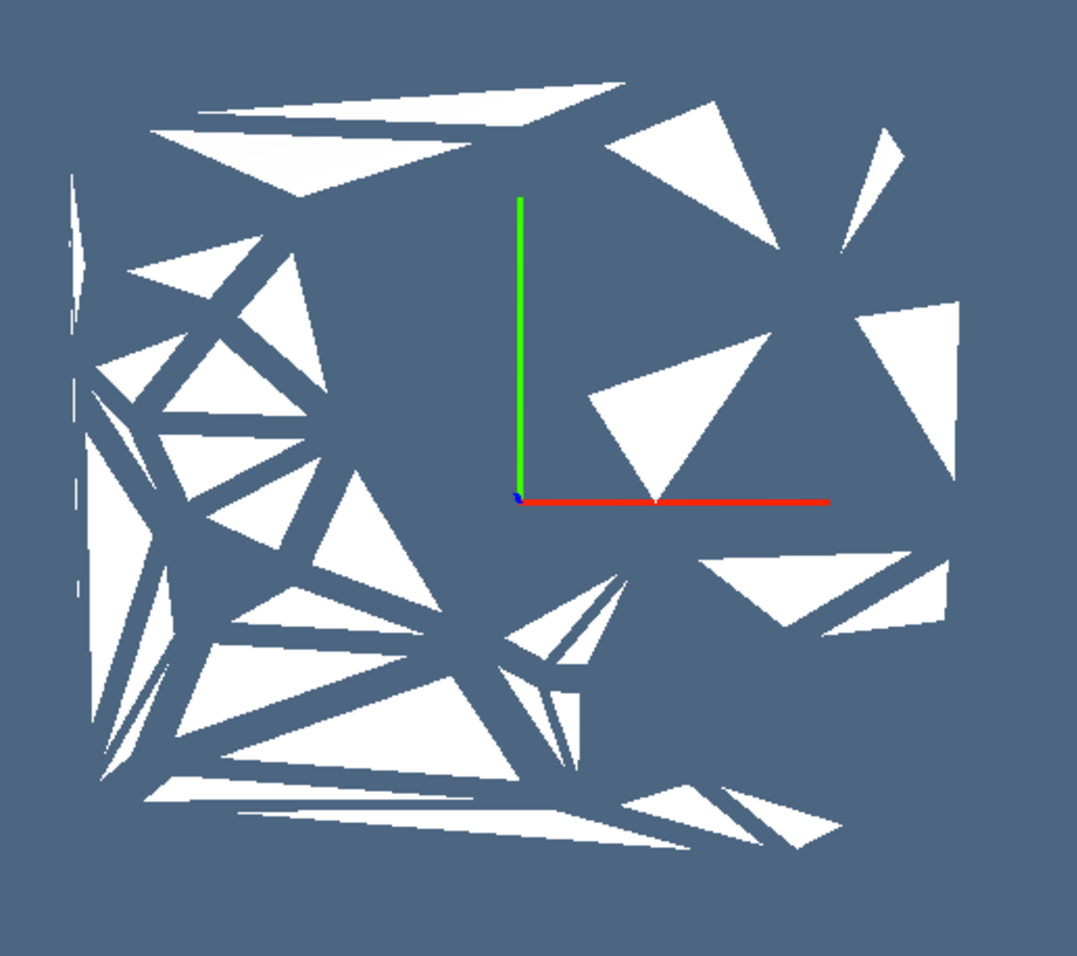
\includegraphics[height=0.25\linewidth,width=0.32\linewidth]{images/tria0} 
   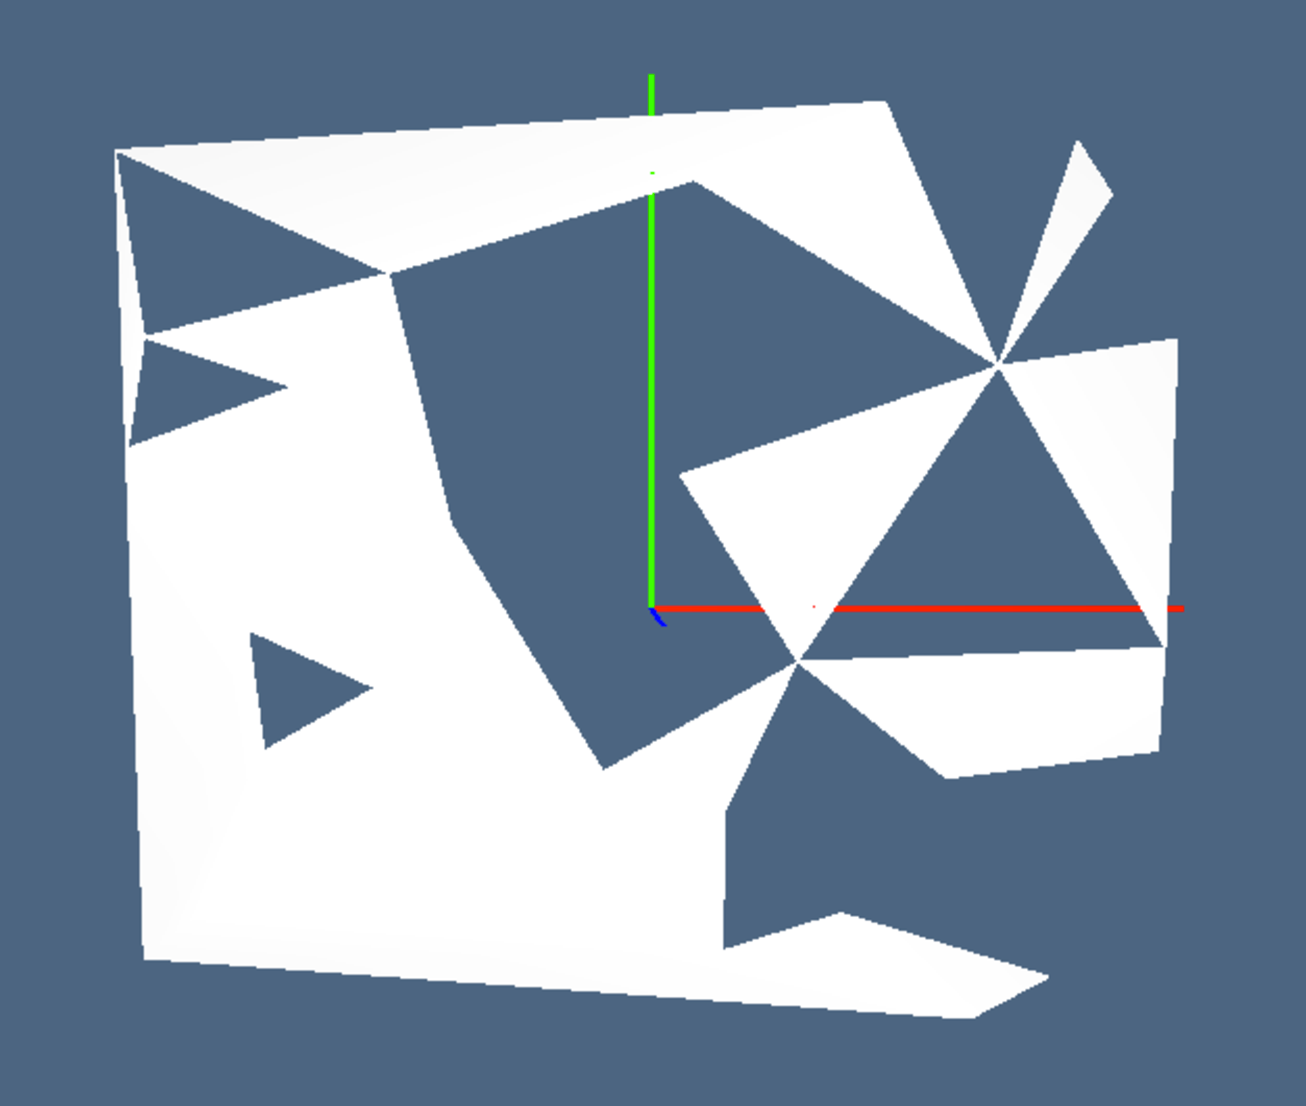
\includegraphics[height=0.25\linewidth,width=0.32\linewidth]{images/tria1} 
   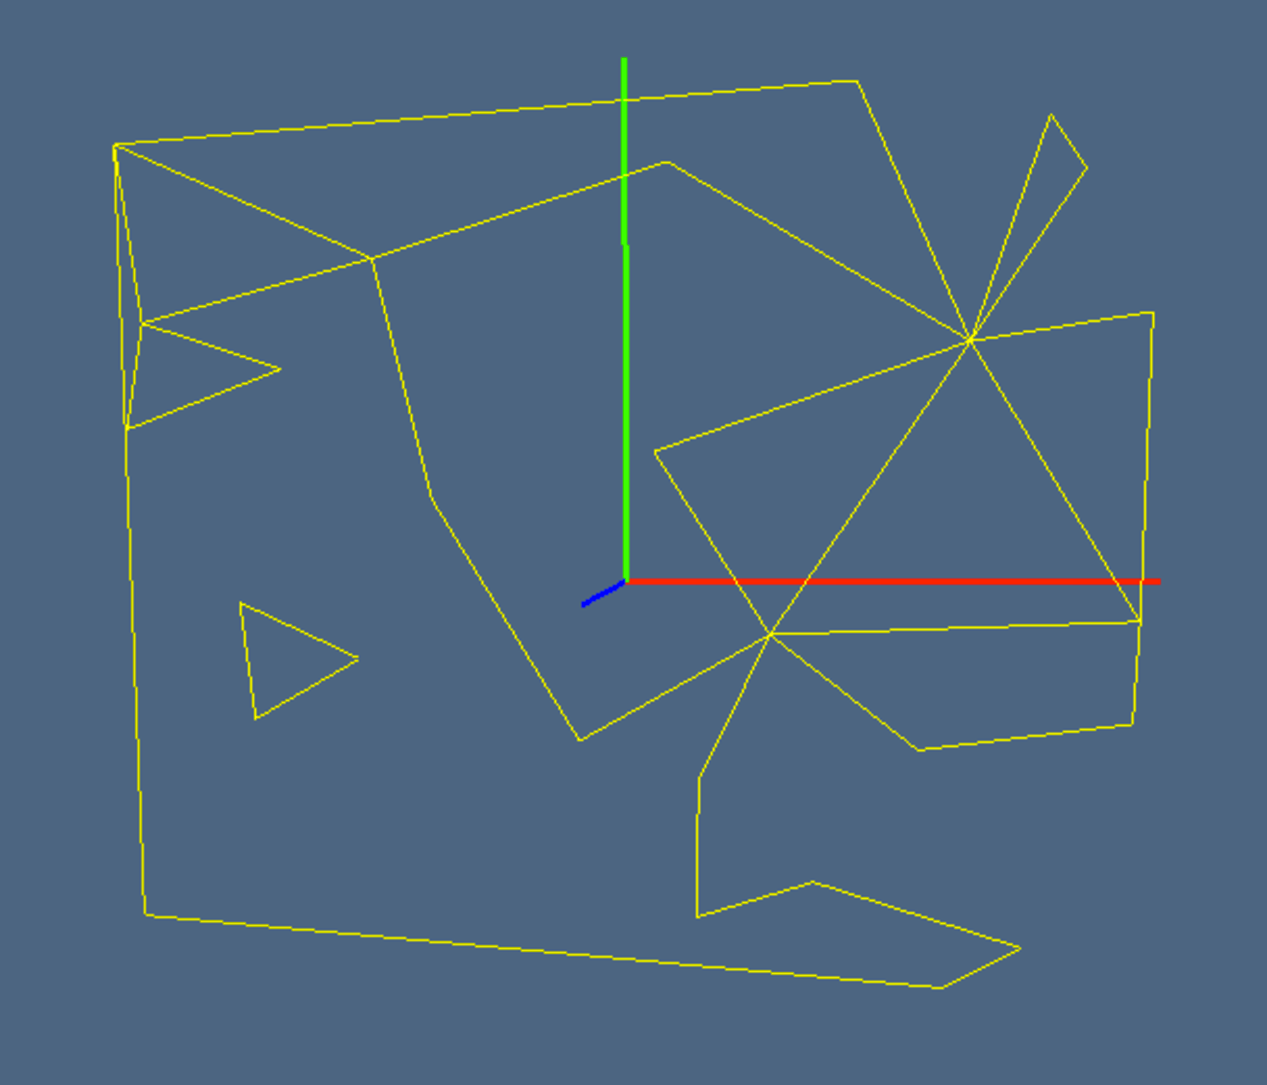
\includegraphics[height=0.25\linewidth,width=0.32\linewidth]{images/tria2} 
   \caption{example caption}
   \label{fig:example}
\end{figure}

%-------------------------------------------------------------------------------
\begin{flushleft} \small
\begin{minipage}{\linewidth} \label{scrap61}
\protect\makebox[0ex][r]{\NWtarget{nuweb27b}{\rule{0ex}{0ex}}\hspace{1em}}$\langle\,$Test for quasi-equilateral triangles\nobreak\ {\footnotesize 27b}$\,\rangle\equiv$
\vspace{-1ex}
\begin{list}{}{} \item
\mbox{}\verb@def quasiEquilateral(tria):@\\
\mbox{}\verb@    a = VECTNORM(VECTDIFF(tria[0:2]))@\\
\mbox{}\verb@    b = VECTNORM(VECTDIFF(tria[1:3]))@\\
\mbox{}\verb@    c = VECTNORM(VECTDIFF([tria[0],tria[2]]))@\\
\mbox{}\verb@    m = max(a,b,c)@\\
\mbox{}\verb@    if m/a < 1.7 and m/b < 1.7 and m/c < 1.7: return True@\\
\mbox{}\verb@    else: return False@\\
\mbox{}\verb@@{\NWsep}
\end{list}
\vspace{-1ex}
\footnotesize\addtolength{\baselineskip}{-1ex}
\begin{list}{}{\setlength{\itemsep}{-\parsep}\setlength{\itemindent}{-\leftmargin}}
\item \NWtxtMacroRefIn\ \NWlink{nuweb27a}{27a}.
\end{list}
\end{minipage}\\[4ex]
\end{flushleft}
%-------------------------------------------------------------------------------

%-------------------------------------------------------------------------------
\begin{flushleft} \small
\begin{minipage}{\linewidth} \label{scrap62}
\protect\makebox[0ex][r]{\NWtarget{nuweb28a}{\rule{0ex}{0ex}}\hspace{1em}}$\langle\,$Generation and selection of random triangles\nobreak\ {\footnotesize 28a}$\,\rangle\equiv$
\vspace{-1ex}
\begin{list}{}{} \item
\mbox{}\verb@verts = np.random.rand(20,2)@\\
\mbox{}\verb@verts = (verts - [0.5,0.5]) * 2@\\
\mbox{}\verb@triangles = Delaunay(verts)@\\
\mbox{}\verb@cells = [ cell for cell in triangles.vertices.tolist()@\\
\mbox{}\verb@         if (not quasiEquilateral([verts[k] for k in cell])) ]@\\
\mbox{}\verb@V, FV = AA(list)(verts), cells@\\
\mbox{}\verb@EV = larSimplexFacets(FV)@\\
\mbox{}\verb@pols2D = MKPOLS((V,FV))@\\
\mbox{}\verb@VIEW(EXPLODE(1.5,1.5,1.5)(pols2D))@\\
\mbox{}\verb@@{\NWsep}
\end{list}
\vspace{-1ex}
\footnotesize\addtolength{\baselineskip}{-1ex}
\begin{list}{}{\setlength{\itemsep}{-\parsep}\setlength{\itemindent}{-\leftmargin}}
\item \NWtxtMacroRefIn\ \NWlink{nuweb27a}{27a}.
\end{list}
\end{minipage}\\[4ex]
\end{flushleft}
%-------------------------------------------------------------------------------

%-------------------------------------------------------------------------------
\begin{flushleft} \small
\begin{minipage}{\linewidth} \label{scrap63}
\protect\makebox[0ex][r]{\NWtarget{nuweb28b}{\rule{0ex}{0ex}}\hspace{1em}}$\langle\,$Boundary computation and visualisation\nobreak\ {\footnotesize 28b}$\,\rangle\equiv$
\vspace{-1ex}
\begin{list}{}{} \item
\mbox{}\verb@boundaryCells_1 = signedBoundaryCells(V,FV,EV)@\\
\mbox{}\verb@print "\nboundaryCells_1 =\n", boundaryCells_1@\\
\mbox{}\verb@def swap(mylist): return [mylist[1]]+[mylist[0]]+mylist[2:]@\\
\mbox{}\verb@boundaryEV = [EV[-k] if k<0 else swap(EV[k]) for k in boundaryCells_1]@\\
\mbox{}\verb@bndry = (V,boundaryEV)@\\
\mbox{}\verb@VIEW(STRUCT(MKPOLS(bndry) + pols2D))@\\
\mbox{}\verb@VIEW(COLOR(RED)(STRUCT(MKPOLS(bndry))))@\\
\mbox{}\verb@@{\NWsep}
\end{list}
\vspace{-1ex}
\footnotesize\addtolength{\baselineskip}{-1ex}
\begin{list}{}{\setlength{\itemsep}{-\parsep}\setlength{\itemindent}{-\leftmargin}}
\item \NWtxtMacroRefIn\ \NWlink{nuweb27a}{27a}.
\end{list}
\end{minipage}\\[4ex]
\end{flushleft}
%-------------------------------------------------------------------------------

%-------------------------------------------------------------------------------
\begin{flushleft} \small
\begin{minipage}{\linewidth} \label{scrap64}
\protect\makebox[0ex][r]{\NWtarget{nuweb28c}{\rule{0ex}{0ex}}\hspace{1em}}$\langle\,$Compute the topologically ordered chain of boundary vertices\nobreak\ {\footnotesize 28c}$\,\rangle\equiv$
\vspace{-1ex}
\begin{list}{}{} \item
\mbox{}\verb@@\\
\mbox{}\verb@@{\NWsep}
\end{list}
\vspace{-1ex}
\footnotesize\addtolength{\baselineskip}{-1ex}
\begin{list}{}{\setlength{\itemsep}{-\parsep}\setlength{\itemindent}{-\leftmargin}}
\item {\NWtxtMacroNoRef}.
\end{list}
\end{minipage}\\[4ex]
\end{flushleft}
%-------------------------------------------------------------------------------

%-------------------------------------------------------------------------------
\begin{flushleft} \small
\begin{minipage}{\linewidth} \label{scrap65}
\protect\makebox[0ex][r]{\NWtarget{nuweb29a}{\rule{0ex}{0ex}}\hspace{1em}}$\langle\,$Decompose a permutation into cycles\nobreak\ {\footnotesize 29a}$\,\rangle\equiv$
\vspace{-1ex}
\begin{list}{}{} \item
\mbox{}\verb@def permutationOrbits(List):@\\
\mbox{}\verb@   d = dict((i,int(x)) for i,x in enumerate(List))@\\
\mbox{}\verb@   out = []@\\
\mbox{}\verb@   while d:@\\
\mbox{}\verb@      x = list(d)[0]@\\
\mbox{}\verb@      orbit = []@\\
\mbox{}\verb@      while x in d:@\\
\mbox{}\verb@         orbit += [x],@\\
\mbox{}\verb@         x = d.pop(x)@\\
\mbox{}\verb@      out += [CAT(orbit)+orbit[0]]@\\
\mbox{}\verb@   return out@\\
\mbox{}\verb@      @\\
\mbox{}\verb@if __name__ == "__main__":@\\
\mbox{}\verb@   print [2, 3, 4, 5, 6, 7, 0, 1]@\\
\mbox{}\verb@   print permutationOrbits([2, 3, 4, 5, 6, 7, 0, 1])@\\
\mbox{}\verb@   print [3,9,8,4,10,7,2,11,6,0,1,5]@\\
\mbox{}\verb@   print permutationOrbits([3,9,8,4,10,7,2,11,6,0,1,5])@\\
\mbox{}\verb@@{\NWsep}
\end{list}
\vspace{-1ex}
\footnotesize\addtolength{\baselineskip}{-1ex}
\begin{list}{}{\setlength{\itemsep}{-\parsep}\setlength{\itemindent}{-\leftmargin}}
\item {\NWtxtMacroNoRef}.
\end{list}
\end{minipage}\\[4ex]
\end{flushleft}
%-------------------------------------------------------------------------------

\subsection{Assemblies of simplices and hypercubes}

%-------------------------------------------------------------------------------
\begin{flushleft} \small
\begin{minipage}{\linewidth} \label{scrap66}
\protect\makebox[0ex][r]{\NWtarget{nuweb29b}{\rule{0ex}{0ex}}\hspace{1em}}\verb@"test/py/larcc/ex7.py"@\nobreak\ {\footnotesize 29b }$\equiv$
\vspace{-1ex}
\begin{list}{}{} \item
\mbox{}\verb@from simplexn import *@\\
\mbox{}\verb@from larcc import *@\\
\mbox{}\verb@from largrid import *@\\
\mbox{}\verb@@\hbox{$\langle\,$Definition of 1-dimensional LAR models\nobreak\ {\footnotesize \NWlink{nuweb30a}{30a}}$\,\rangle$}\verb@@\\
\mbox{}\verb@@\hbox{$\langle\,$Assembly generation of squares and triangles\nobreak\ {\footnotesize \NWlink{nuweb30b}{30b}}$\,\rangle$}\verb@@\\
\mbox{}\verb@@\hbox{$\langle\,$Assembly generation of cubes and tetrahedra\nobreak\ {\footnotesize \NWlink{nuweb30c}{30c}}$\,\rangle$}\verb@@\\
\mbox{}\verb@@{\NWsep}
\end{list}
\vspace{-2ex}
\end{minipage}\\[4ex]
\end{flushleft}
%-------------------------------------------------------------------------------

\begin{figure}[htbp] %  figure placement: here, top, bottom, or page
   \centering
   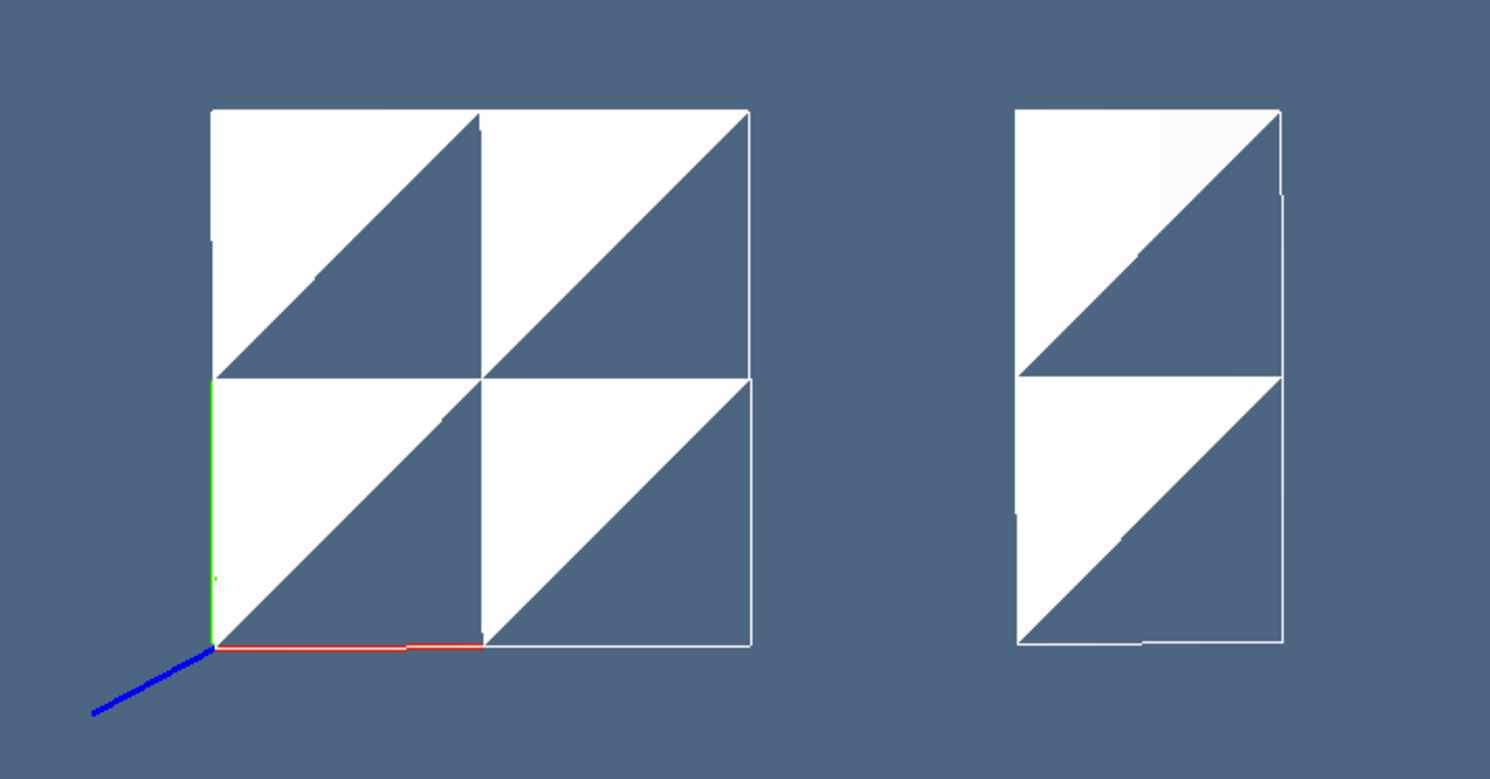
\includegraphics[width=0.405\linewidth]{images/assembly1} 
   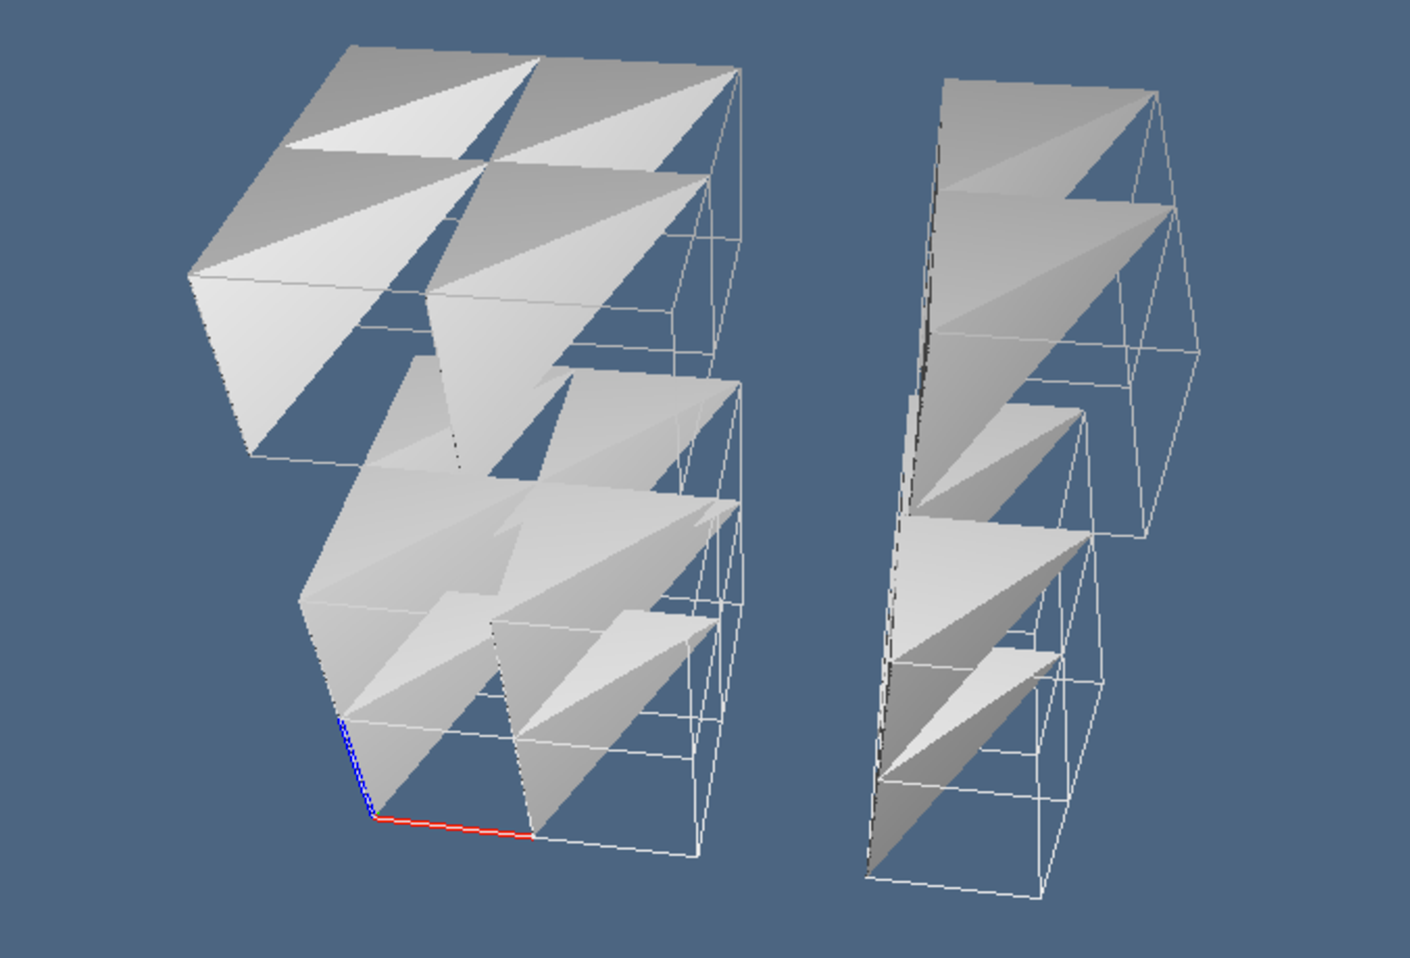
\includegraphics[width=0.315\linewidth]{images/assembly2} 
   \caption{(a) Assemblies of squares and triangles; (b) assembly of cubes and tetrahedra.}
   \label{fig:example}
\end{figure}

%-------------------------------------------------------------------------------
\begin{flushleft} \small
\begin{minipage}{\linewidth} \label{scrap67}
\protect\makebox[0ex][r]{\NWtarget{nuweb30a}{\rule{0ex}{0ex}}\hspace{1em}}$\langle\,$Definition of 1-dimensional LAR models\nobreak\ {\footnotesize 30a}$\,\rangle\equiv$
\vspace{-1ex}
\begin{list}{}{} \item
\mbox{}\verb@geom_0,topol_0 = [[0.],[1.],[2.],[3.],[4.]],[[0,1],[1,2],[3,4]]@\\
\mbox{}\verb@geom_1,topol_1 = [[0.],[1.],[2.]], [[0,1],[1,2]]@\\
\mbox{}\verb@mod_0 = (geom_0,topol_0)@\\
\mbox{}\verb@mod_1 = (geom_1,topol_1)@\\
\mbox{}\verb@@{\NWsep}
\end{list}
\vspace{-1ex}
\footnotesize\addtolength{\baselineskip}{-1ex}
\begin{list}{}{\setlength{\itemsep}{-\parsep}\setlength{\itemindent}{-\leftmargin}}
\item \NWtxtMacroRefIn\ \NWlink{nuweb29b}{29b}.
\end{list}
\end{minipage}\\[4ex]
\end{flushleft}
%-------------------------------------------------------------------------------

%-------------------------------------------------------------------------------
\begin{flushleft} \small
\begin{minipage}{\linewidth} \label{scrap68}
\protect\makebox[0ex][r]{\NWtarget{nuweb30b}{\rule{0ex}{0ex}}\hspace{1em}}$\langle\,$Assembly generation of squares and triangles\nobreak\ {\footnotesize 30b}$\,\rangle\equiv$
\vspace{-1ex}
\begin{list}{}{} \item
\mbox{}\verb@squares = larModelProduct([mod_0,mod_1])@\\
\mbox{}\verb@V,FV = squares@\\
\mbox{}\verb@simplices = pivotSimplices(V,FV,d=2)@\\
\mbox{}\verb@VIEW(STRUCT([ MKPOL([V,AA(AA(C(SUM)(1)))(simplices),[]]),@\\
\mbox{}\verb@              SKEL_1(STRUCT(MKPOLS((V,FV)))) ]))@\\
\mbox{}\verb@@{\NWsep}
\end{list}
\vspace{-1ex}
\footnotesize\addtolength{\baselineskip}{-1ex}
\begin{list}{}{\setlength{\itemsep}{-\parsep}\setlength{\itemindent}{-\leftmargin}}
\item \NWtxtMacroRefIn\ \NWlink{nuweb29b}{29b}.
\end{list}
\end{minipage}\\[4ex]
\end{flushleft}
%-------------------------------------------------------------------------------

%-------------------------------------------------------------------------------
\begin{flushleft} \small
\begin{minipage}{\linewidth} \label{scrap69}
\protect\makebox[0ex][r]{\NWtarget{nuweb30c}{\rule{0ex}{0ex}}\hspace{1em}}$\langle\,$Assembly generation of cubes and tetrahedra\nobreak\ {\footnotesize 30c}$\,\rangle\equiv$
\vspace{-1ex}
\begin{list}{}{} \item
\mbox{}\verb@cubes = larModelProduct([squares,mod_0])@\\
\mbox{}\verb@V,CV = cubes@\\
\mbox{}\verb@simplices = pivotSimplices(V,CV,d=3)@\\
\mbox{}\verb@VIEW(STRUCT([ MKPOL([V,AA(AA(C(SUM)(1)))(simplices),[]]),@\\
\mbox{}\verb@           SKEL_1(STRUCT(MKPOLS((V,CV)))) ]))@\\
\mbox{}\verb@@{\NWsep}
\end{list}
\vspace{-1ex}
\footnotesize\addtolength{\baselineskip}{-1ex}
\begin{list}{}{\setlength{\itemsep}{-\parsep}\setlength{\itemindent}{-\leftmargin}}
\item \NWtxtMacroRefIn\ \NWlink{nuweb29b}{29b}.
\end{list}
\end{minipage}\\[4ex]
\end{flushleft}
%-------------------------------------------------------------------------------







\bibliographystyle{amsalpha}
\bibliography{larcc}

\end{document}
